This section provides background on operating system terminology such
as processes, threads, memory protection, virtualization and hypervisors.

\section{Processes and Threads}
\paragraph{Process:} A process can be viewed both as a program in execution
and as an abstraction of a processor. Each process has its own address
space~\cite{Galvin}.

\paragraph{Threads:} A process has either a single or multiple threads
sharing its address space. Each thread represents a separate flow of
control~\cite{Galvin}.

A thread is also called a light-weight process. The implementation of
threads and processes differs between operating systems. A process's 
threads share resources such as code and data segments, whereas 
different processes do not share such resources.
\begin{figure}[!ht]
    \centering
    \begin{subfigure}[b]{0.45\textwidth}
	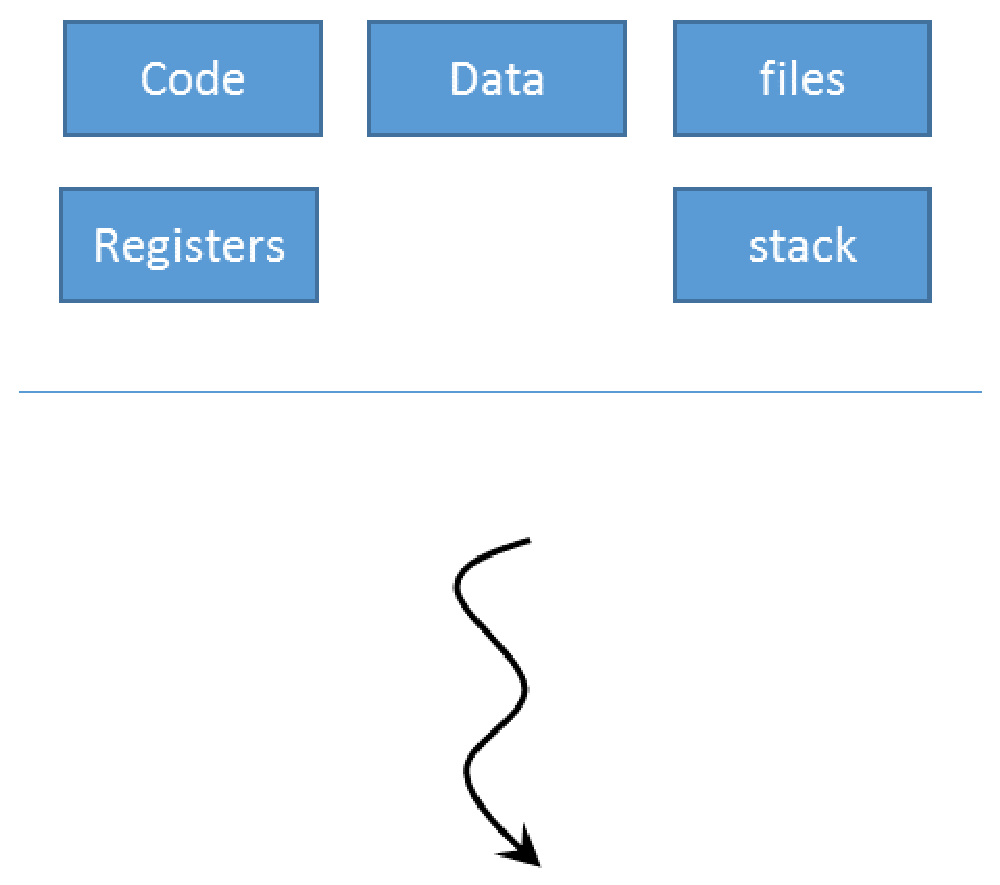
\includegraphics[scale=.25]{thread1}
	\caption{Single-threaded process}
	\label{fig:thread1}
    \end{subfigure}
	\hfill
    \begin{subfigure}[b]{0.45\textwidth}
	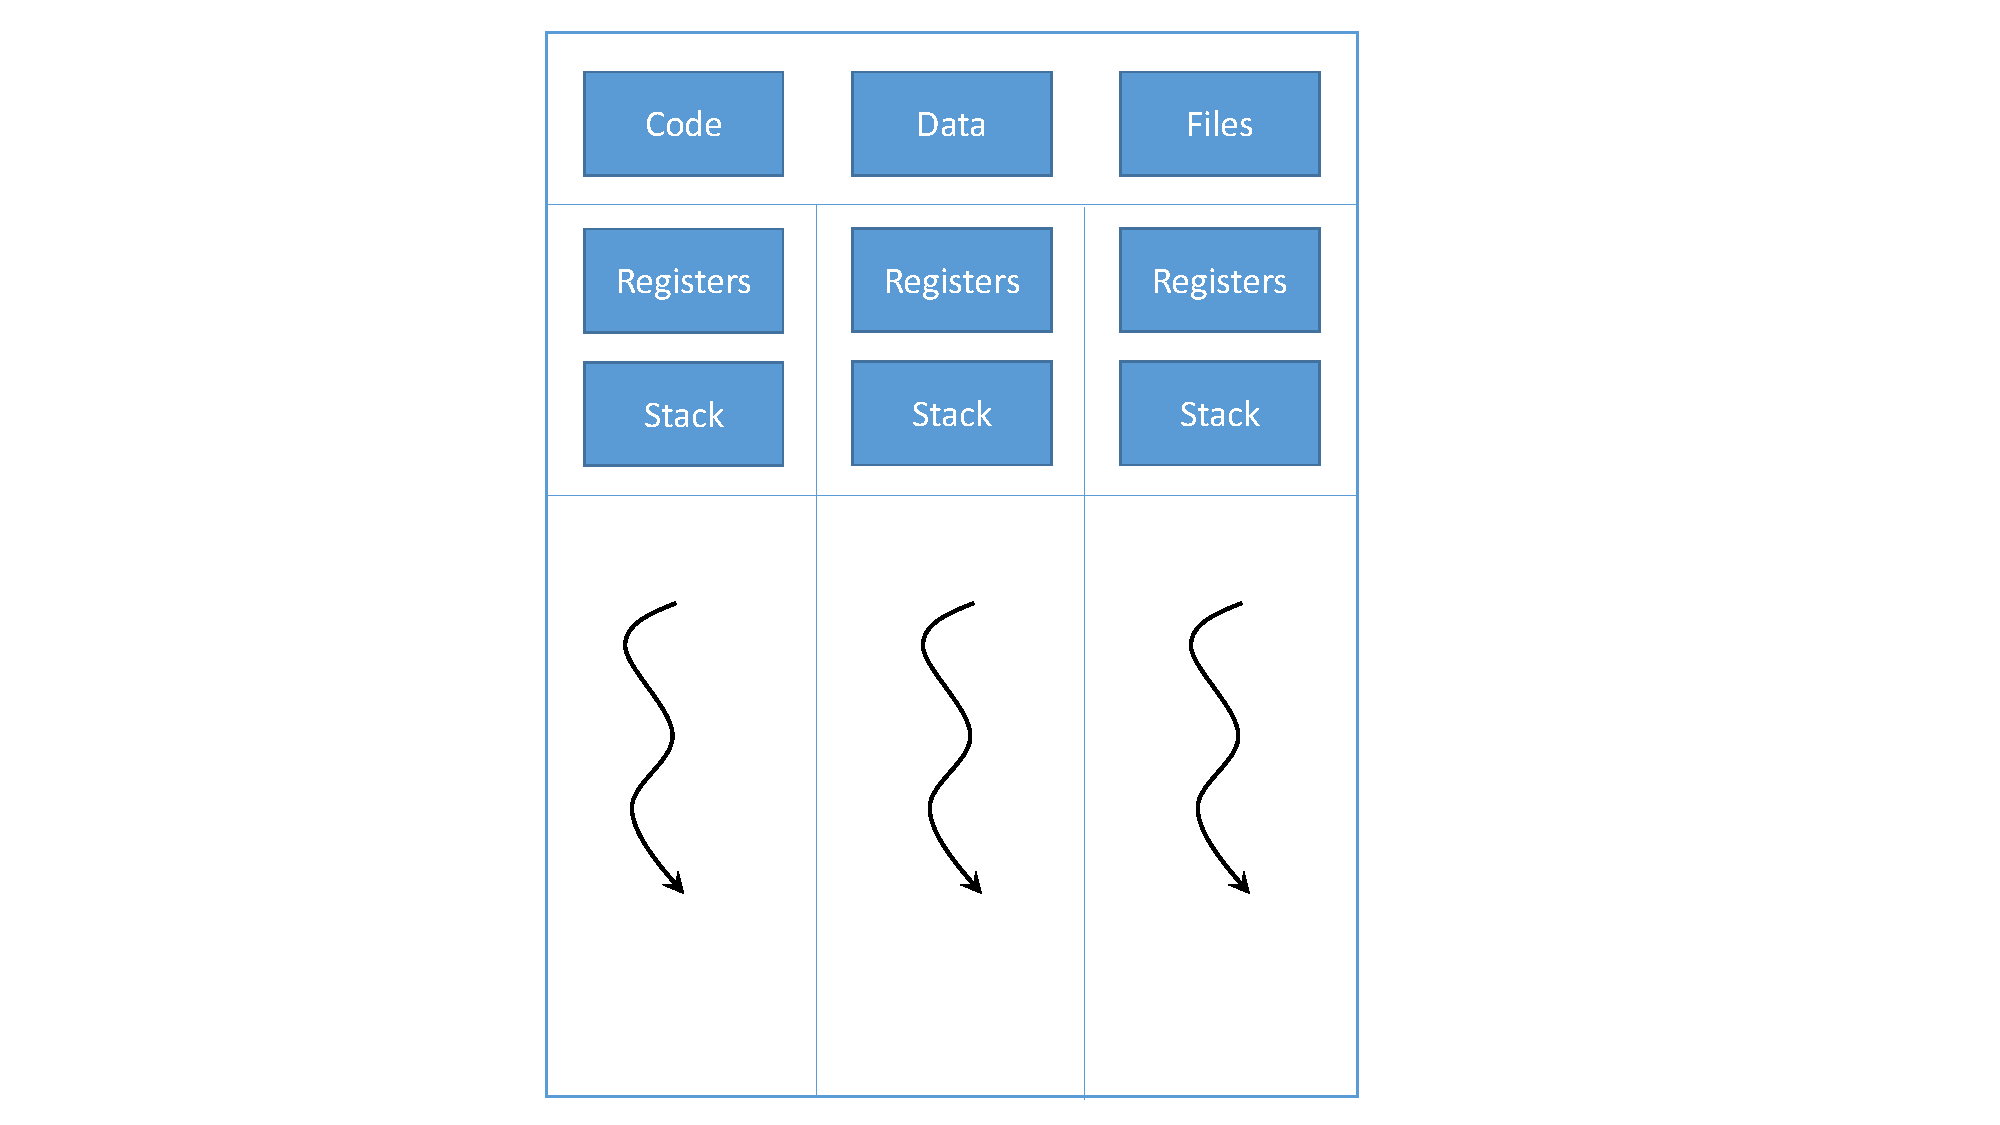
\includegraphics[scale=.25]{thread2}
	\caption{Multithreaded process}
	\label{fig:thread2}
    \end{subfigure}
    \caption{Thread}\label{fig:threads}
\end{figure}

\section{Context Switch}
Multiple threads typically employ time division multiplexing when sharing
a single processor.  In time division multiplexing, the processor switches
between executing threads, interleaving their execution. The process of 
switching between threads is called a context switch. Continuous context switching
creates the impression for the user that threads and processes are
running concurrently. On multiprocessor systems, threads can also run
simultaneously on multiple processors, each of which may perform time
division multiplexing.

During a context switch the state of a thread is saved so that its
execution can be resumed from the same point at a later time. The
composition of the saved state is determined by the processor and the operating system
~\cite{Galvin}. The costs of context switches can be divided into direct and
indirect costs. The direct cost is the time required to save and restore
processor registers, execute the scheduler code, flush TLB entries and
to flush the processor pipeline. Indirect costs include subsequent cache miss 
penalties that are due to processor 
pollution~\cite{Soares+:osdi10, Li:2007:QCC:1281700.1281702}.

\section{Spinlocks}
In uniprocessor and multiprocessor environments, a context switch takes a
significant amount of time.  In a multi-processor environment, it may be more
efficient for each process to keep its own CPU and spin while waiting
for a resource.

A spinlock is a locking mechanism designed to work in a multiprocessor
environment. A spinlock causes a thread that is trying to acquire lock
to spin if the lock is not immediately available~\cite{Bovet:2005:ULK:1077084}.

\textbf{Adaptive Spinning} is a spinlock optimization technique. 
After unsuccessfully spinning for a set threshold amount of time, a thread
will block as for regular locks.
In the adaptive spinning technique, the spinning threshold is determined by
an algorithm based on the rate of successes and failures of recent spinning
attempts to acquire the lock.  Adaptive spinning helps threads to avoid
spinning in conditions where it would not be beneficial.

\section{Device Driver}
\label{sec:device driver}

A device driver is a program that provides a software interface to a
particular hardware device. It enables the operating system and other
programs to access its hardware functions. Device drivers are hardware
dependent and operating system specific.  A driver issues commands to 
a device in response to system calls requested by user programs.
After executing these commands,
the device sends data back to the driver. The driver informs the caller by 
invoking callback routines after receiving the data. The Linux
kernel distinguishes between three device types: character devices,
block devices, and network interfaces.

\begin{figure}[!ht]
\centering
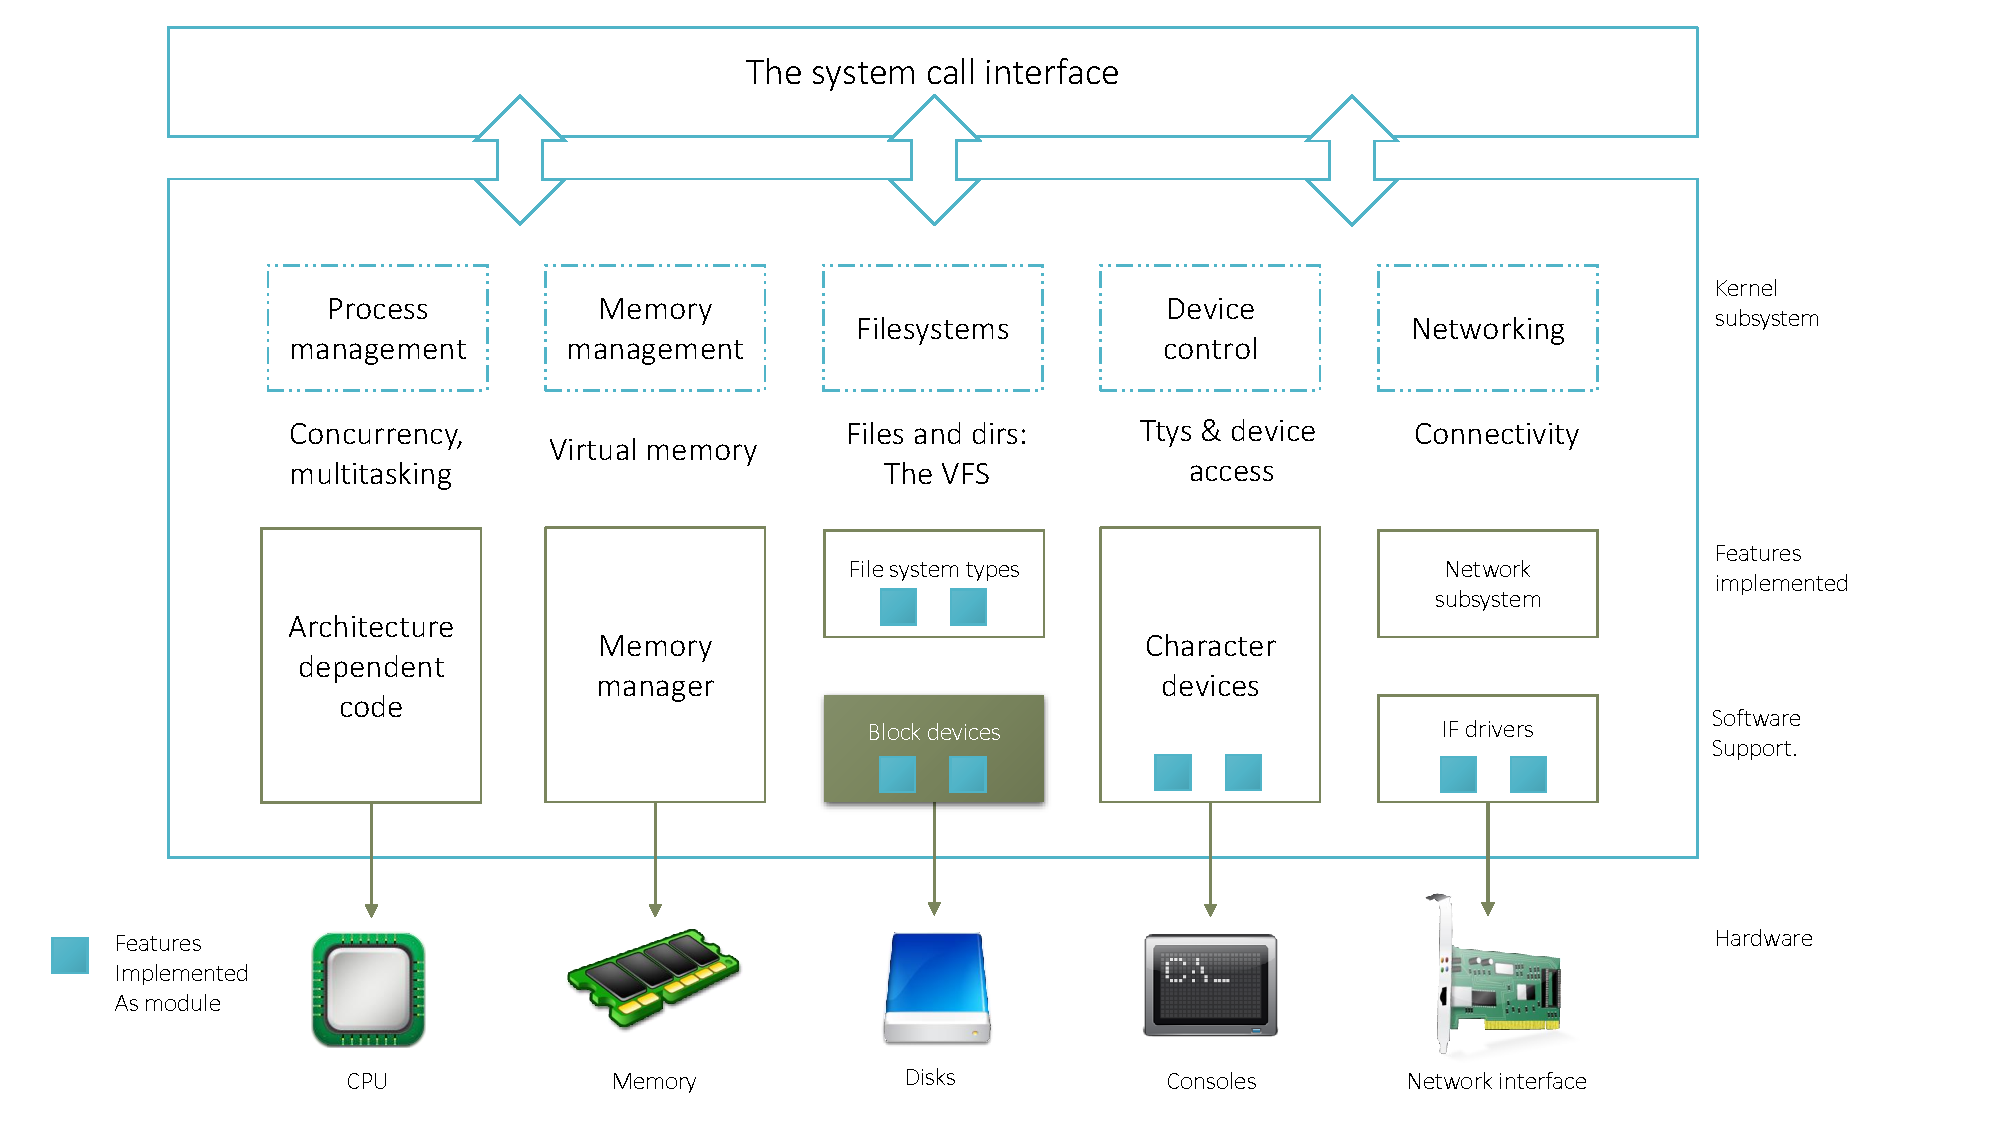
\includegraphics[scale=.5 ]{kernel}
\caption{Split view of a kernel}
\label{fig:kernel}
\end{figure}

\paragraph{Character devices:} A character device can be accessed as
a stream of bytes. A character driver usually implements at least the
open, close, read, and write functions. The text console (/dev/console)
and the serial ports (/dev/ttyS0) are examples of character devices.

\paragraph{Network Interfaces:} A network interface is a device that
is able to exchange data with other hosts. Usually, a network interface
is a hardware device, but it can be a software device such as the loopback
interface.

\paragraph{Block Devices:} Unlike character devices, block devices
are accessed as blocks of data. Whereas most Unix implementations
support only I/O operations that involve entire blocks,
Linux also allows applications to read and write individual bytes within
a block. As a result, in Linux, block and char devices
differ only in the way data is managed internally by the kernel. 
Examples of block devices are disks and CDs~\cite{Corbet:2005:LDD:1209083}.

\subsection*{Block Device Driver}
\subsubsection*{Request processing in a block device driver}

\label{subsec:request queue}
A block device driver maintains a request queue to store read and write
requests. In order to initialize a request queue, a spinlock and a
request function pointer is required.  The request function forms
the central part of the block device driver. Requests are added to
the request queue when a request is made by higher level code in the
Linux kernel, such as a file system. A block device driver's
request function is called after receiving a new request. The request function
must remove all requests from the head of the request queue and send
them to the block device for execution. The Linux kernel acquires a
spinlock before calling the request function and releases it after
returning. As a result, a request function runs in a mutually 
exclusive context~\cite{Corbet:2005:LDD:1209083}.

A request is a linked list of \texttt{struct bio} objects. The \texttt{bio} 
structure contains all the information required to execute a read or write
operation on a block device. The block I/O code receives the bio
structure from the higher level code in the Linux kernel. The
block I/O code may add the received bio structure to an existing
request~\cite{Corbet:2005:LDD:1209083}, if any, or it must create
a new request.

Each bio structure in a request describes the low level block I/O
request. If possible, the Linux kernel merges several independent
requests to form one block I/O request. Usually the kernel combines
multiple requests if they require access to adjacent sectors on
the disk. However, it never combines read and write requests.

\section{Memory Protection}

The memory protection mechanism of a computer system controls
access to resources. The goal of memory protection is to prevent
malicious misuse of the system by users or programs. Memory
protection also ensures that a resource is used in accordance
with the system policies. In addition, it also helps to
ensure that errant programs cause minimal damage~\cite{Galvin,
Graham:1971:PPP:1478873.1478928}. Subsection~\ref{subsec:user level}
and subsection~\ref{subsec:kernel level} explain the policies implemented
at kernel level and user level.

\subsection{User Level}
\label{subsec:user level}
%
% ............. CONTINUE HERE
%

Typically in a monolithic kernel, the lowest \texttt{X Gb} of memory is
reserved for user processes. The upper \texttt{Virtual Memory size - X Gb}
is reserved for the kernel. The kernel puts its private data structures
in the upper memory and always accesses them at the same virtual address.

\begin{figure}[!ht]
\centering
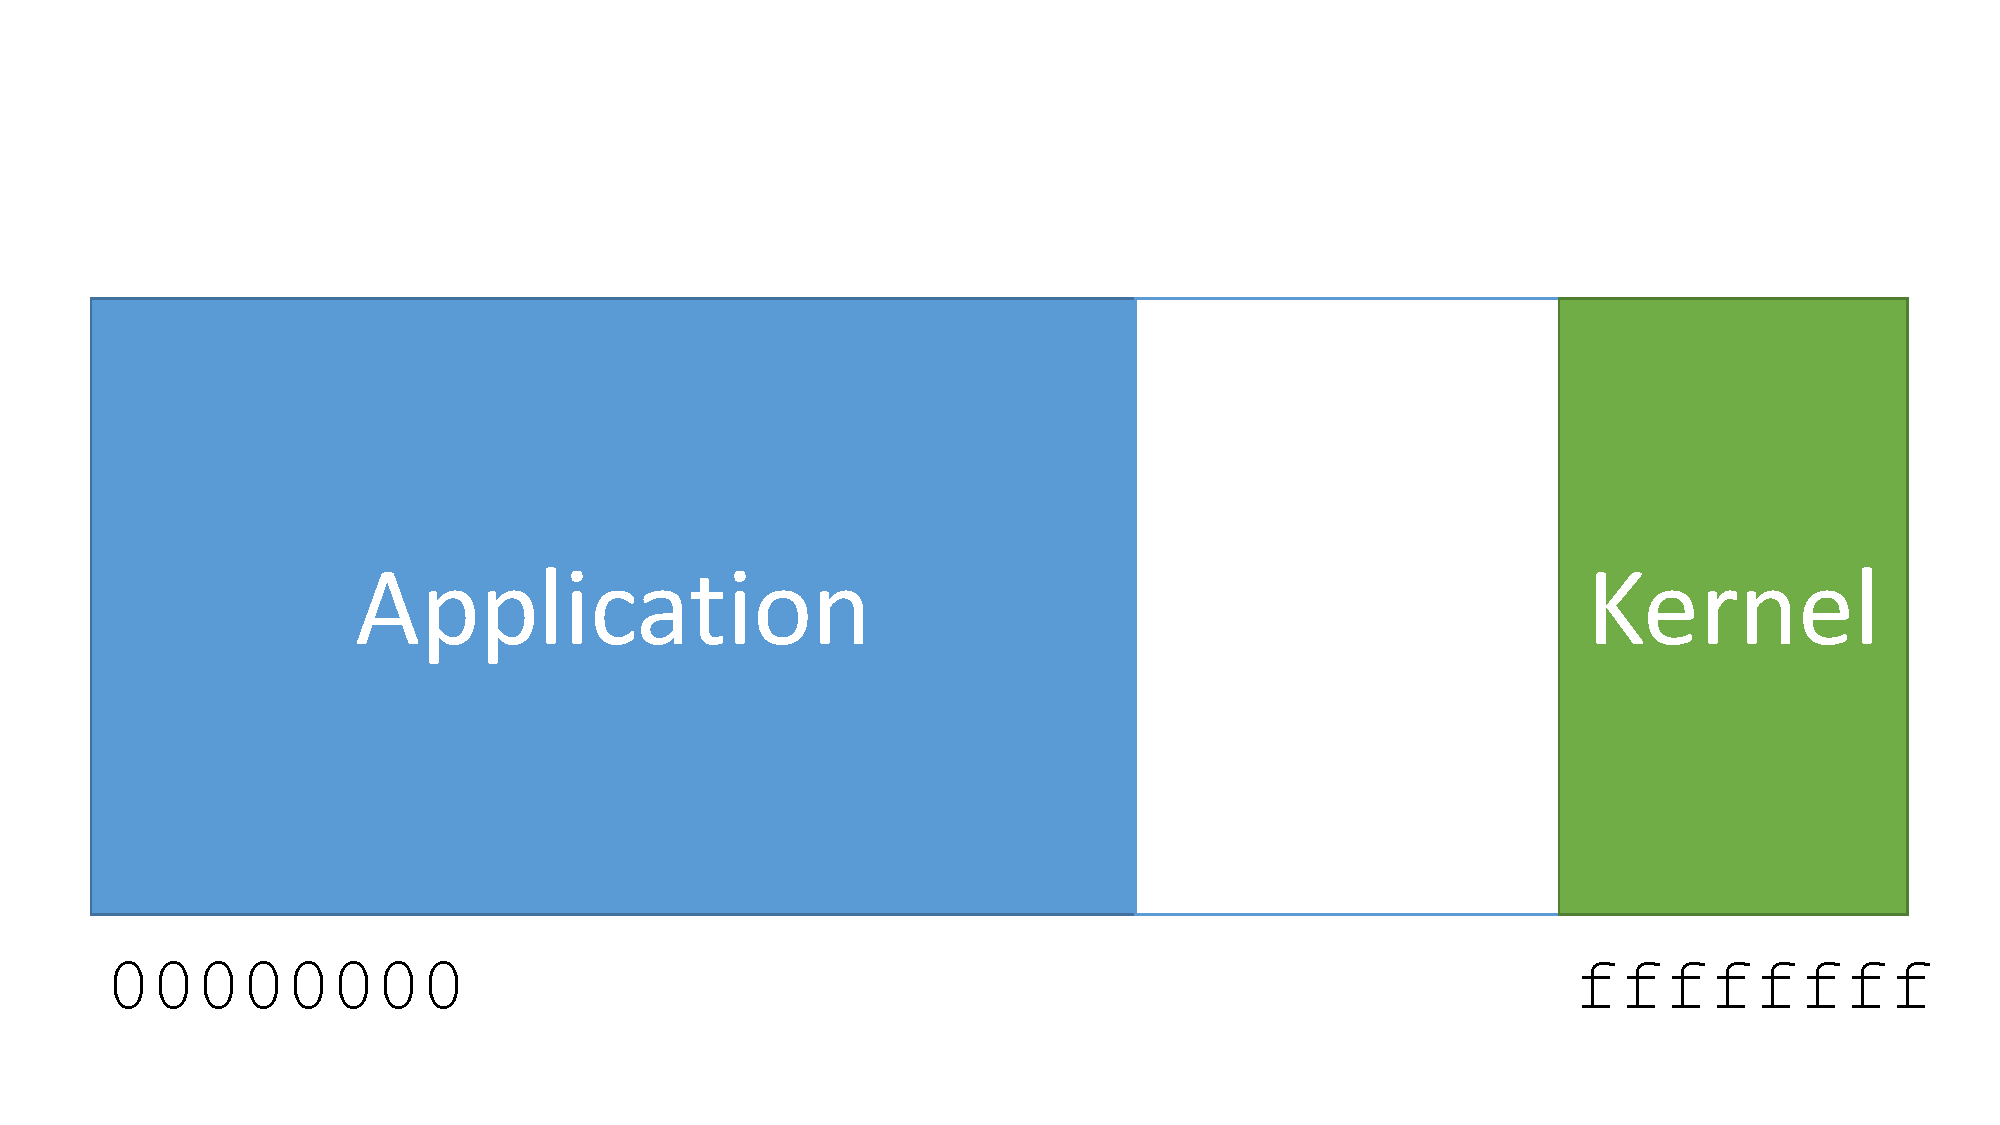
\includegraphics[scale=.25 ]{memory_map}
\caption{Physical memory}
\label{fig:memmap}
\end{figure}

At the user space, each application runs as a separate process. Each
process is associated with an address space and believes that it owns the
entire memory, starting with the virtual address 0. However, a translation
table translates every memory reference by these processes from virtual
to physical addresses. The translation table maintains \texttt{$<$base,
bound$>$} entries. If a process tries to access virtual address that
is outside the \texttt{base + bound} address, then an error is reported
by the operating system, otherwise the physical address \texttt{base +
virtual address} is returned. This allows multiple processes to be run in
the memory with protection. Since address translation provides protection,
a process cannot access addresses outside its address space.

Consider the example shown in Figure~\ref{fig:User space}.
\begin{enumerate}
\item This system is running 3 different user processes
\item One of the processes encounters a bug and tries to access a memory address outside its address space
\item Access to the address is restricted by the memory protection mechanism
\begin{figure}[!ht]
    \centering
    \begin{subfigure}[b]{0.49\textwidth}
	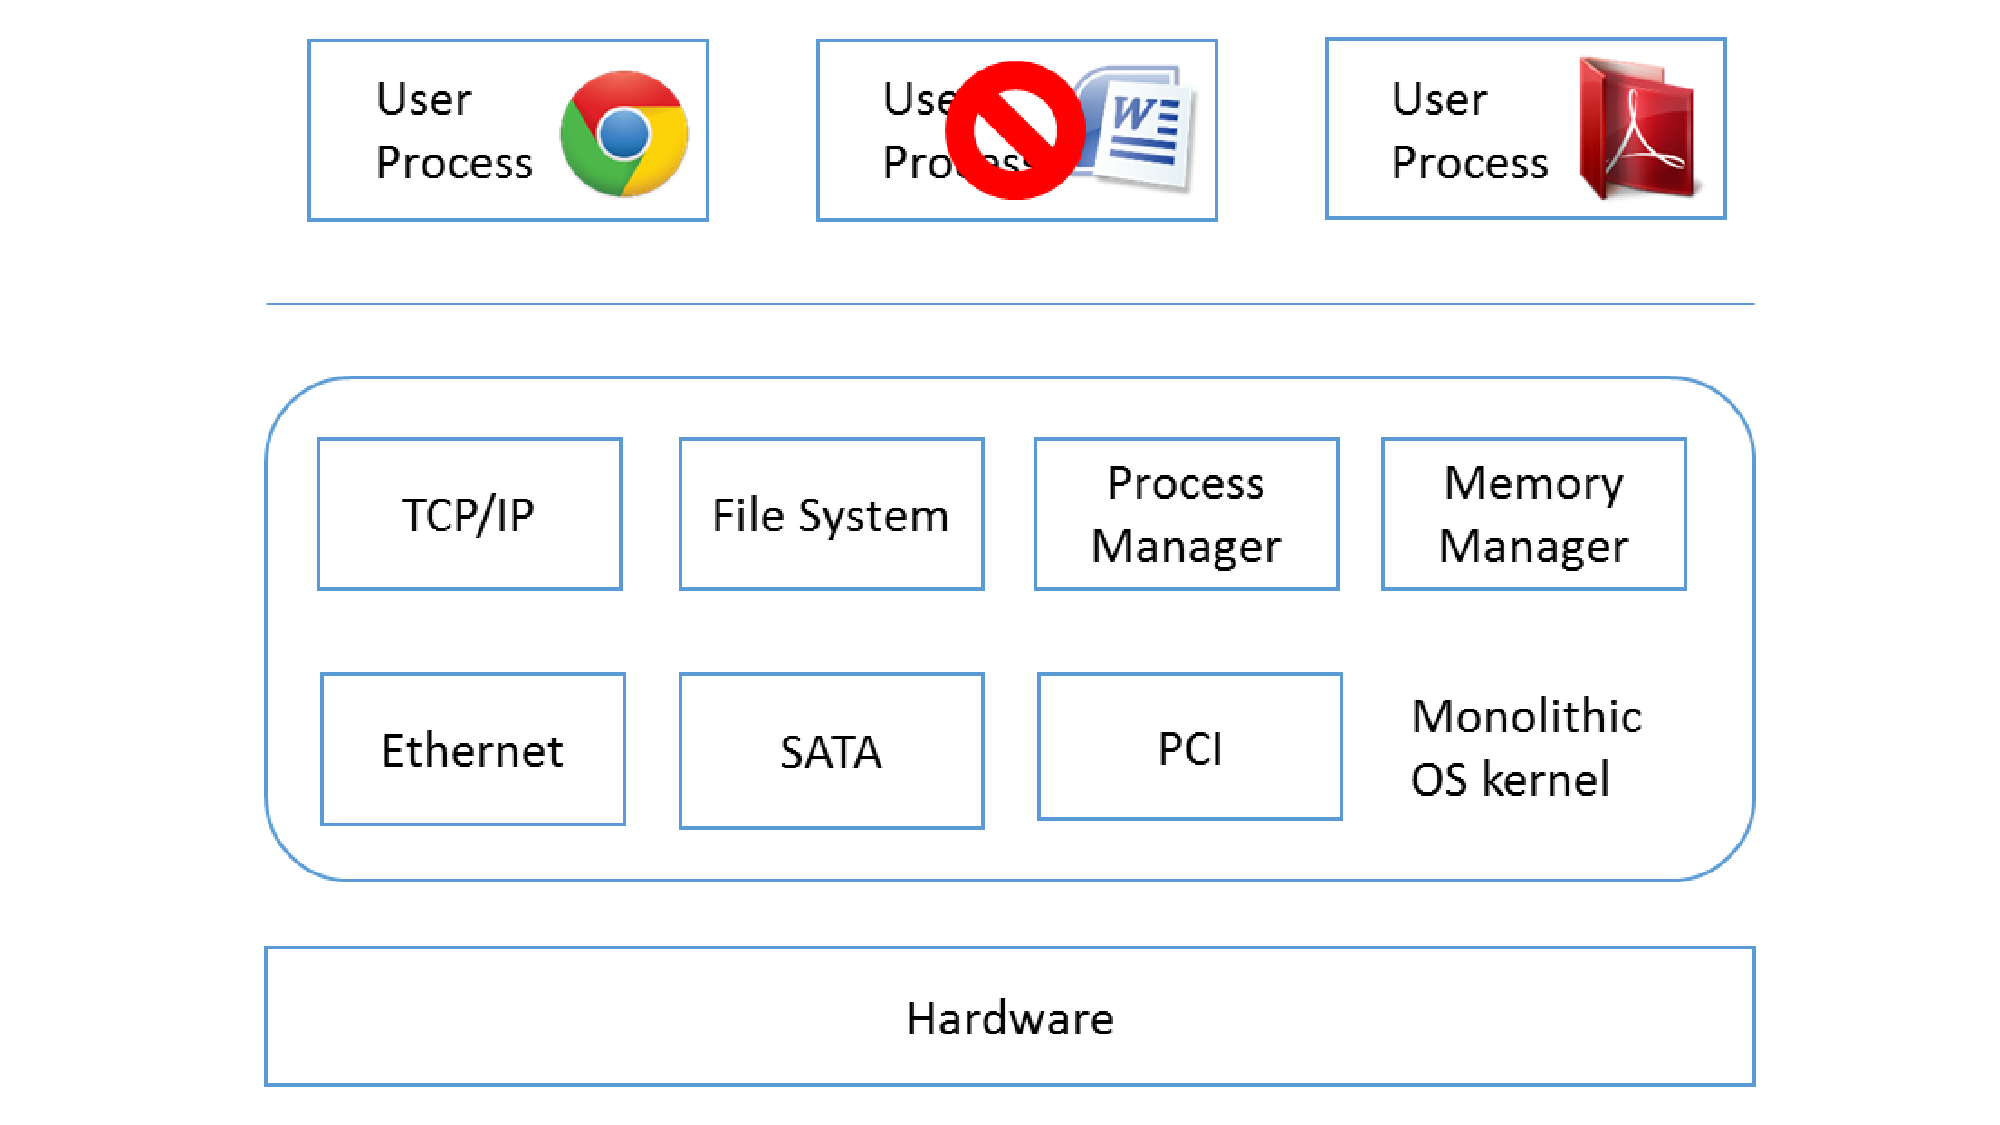
\includegraphics[scale=.25]{user-space-1}
	\caption{A process encounters a bug}
    \end{subfigure}
	\hfill
    \begin{subfigure}[b]{0.49\textwidth}
	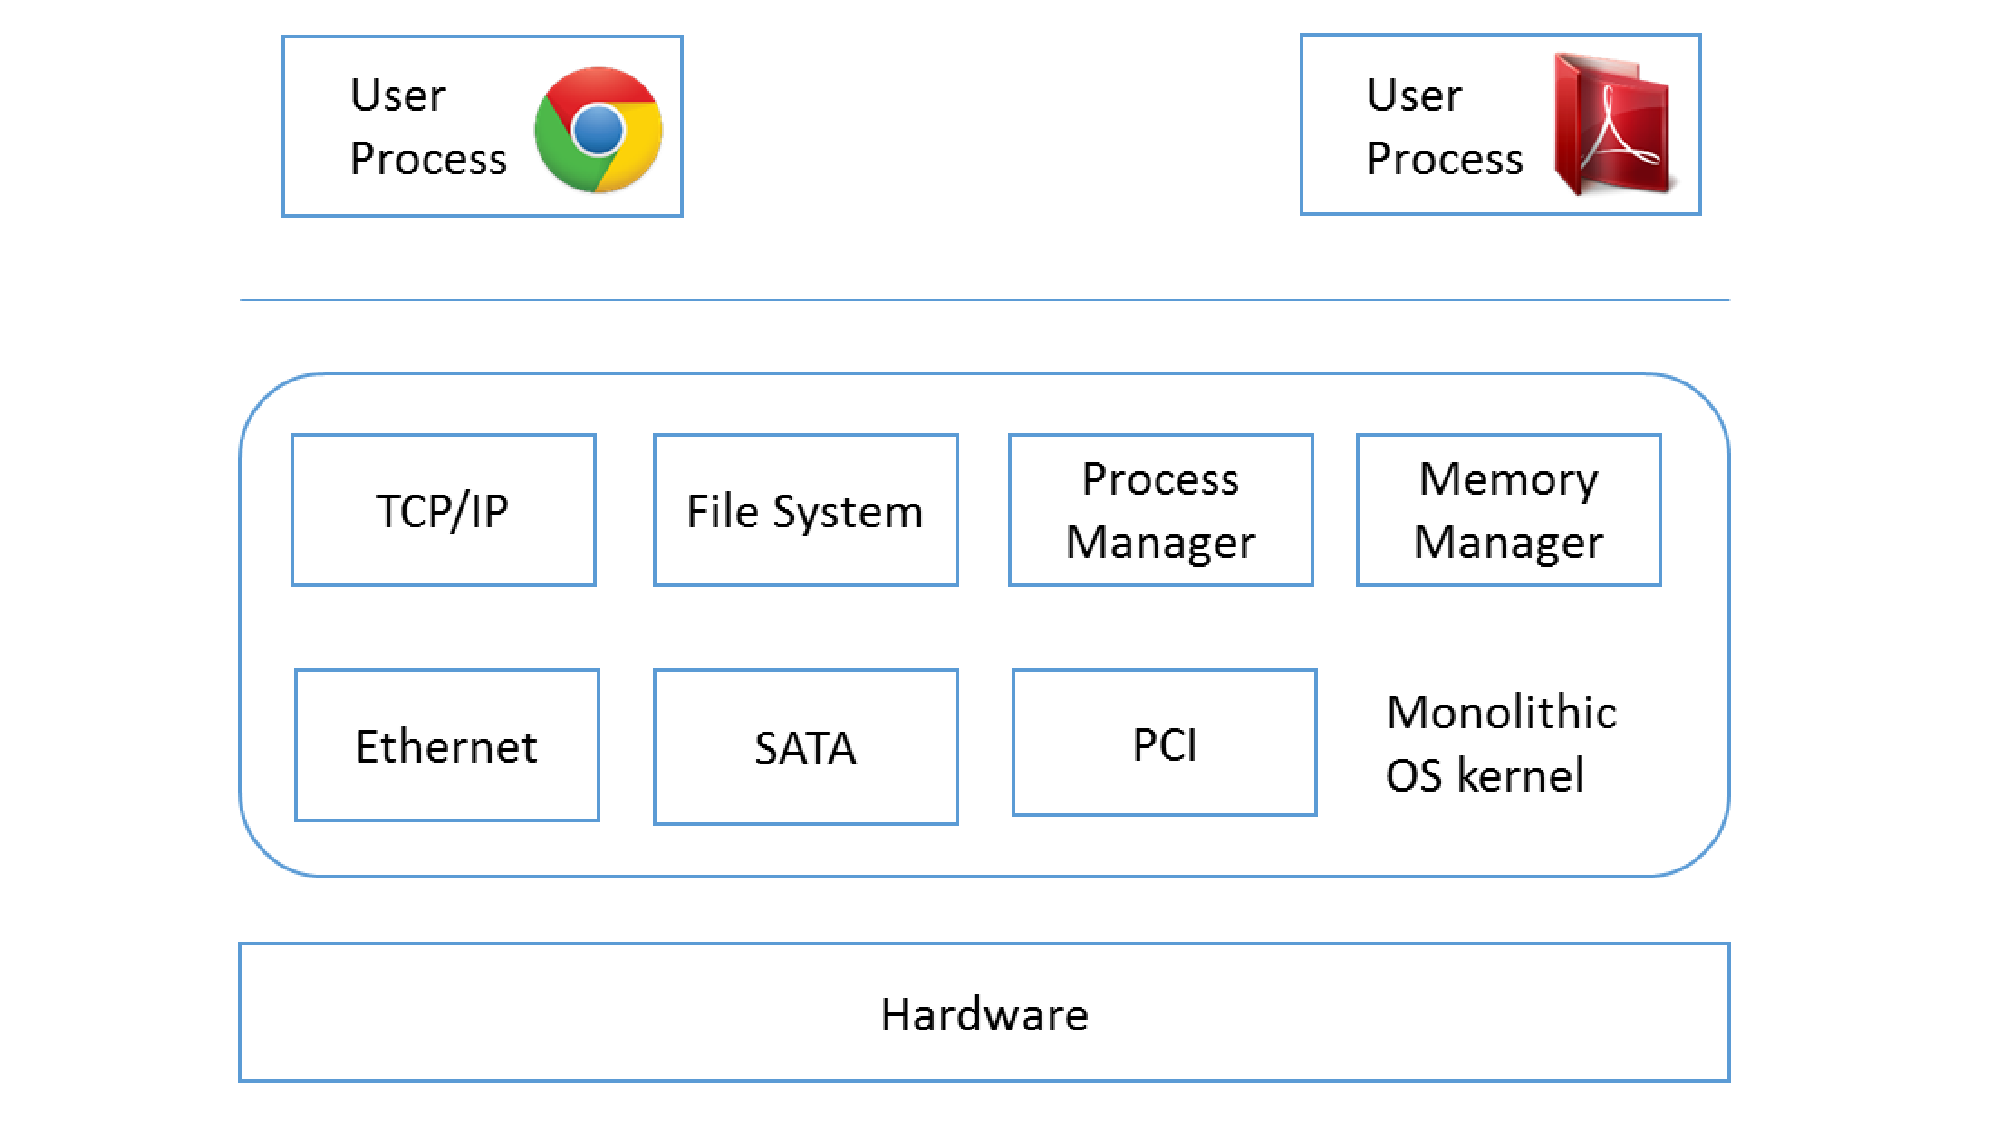
\includegraphics[scale=.25]{user-space-2}
	\caption{Other user processes are not affected}
    \end{subfigure}
    \caption{User level memory protection}\label{fig:User space}
\end{figure}
\end{enumerate}

\subsection{Kernel Level}
\label{subsec:kernel level}
This sections explains how memory is managed at kernel level. 

In a Linux kernel, virtual memory is divided into pages and physical memory is divided into blocks called as page frames. Linux kernel uses a data structure called page table to store virtual memory to physical memory mapping information. Kernel reserves upper virtual memory for its internal use. The page table entries of this region are marked as protected so that pages are not visible or modifiable in the user mode. However, at kernel level any code running at priviledged level can access the kernel memory. Hence a kernel component can access, and potentially, corrupt any kernel data structures.

Consider the example shown in Figure~\ref{fig:Kernel space}
\begin{enumerate}
\item The system runs 3 different processes in the user space and has different kernel components running in kernel space.
\item The network driver hits a bug, and corrupts kernel data structures. The corruption might lead to a system crash.
\end{enumerate}
\begin{figure}[!ht]
    \centering
    \begin{subfigure}[b]{0.49\textwidth}
	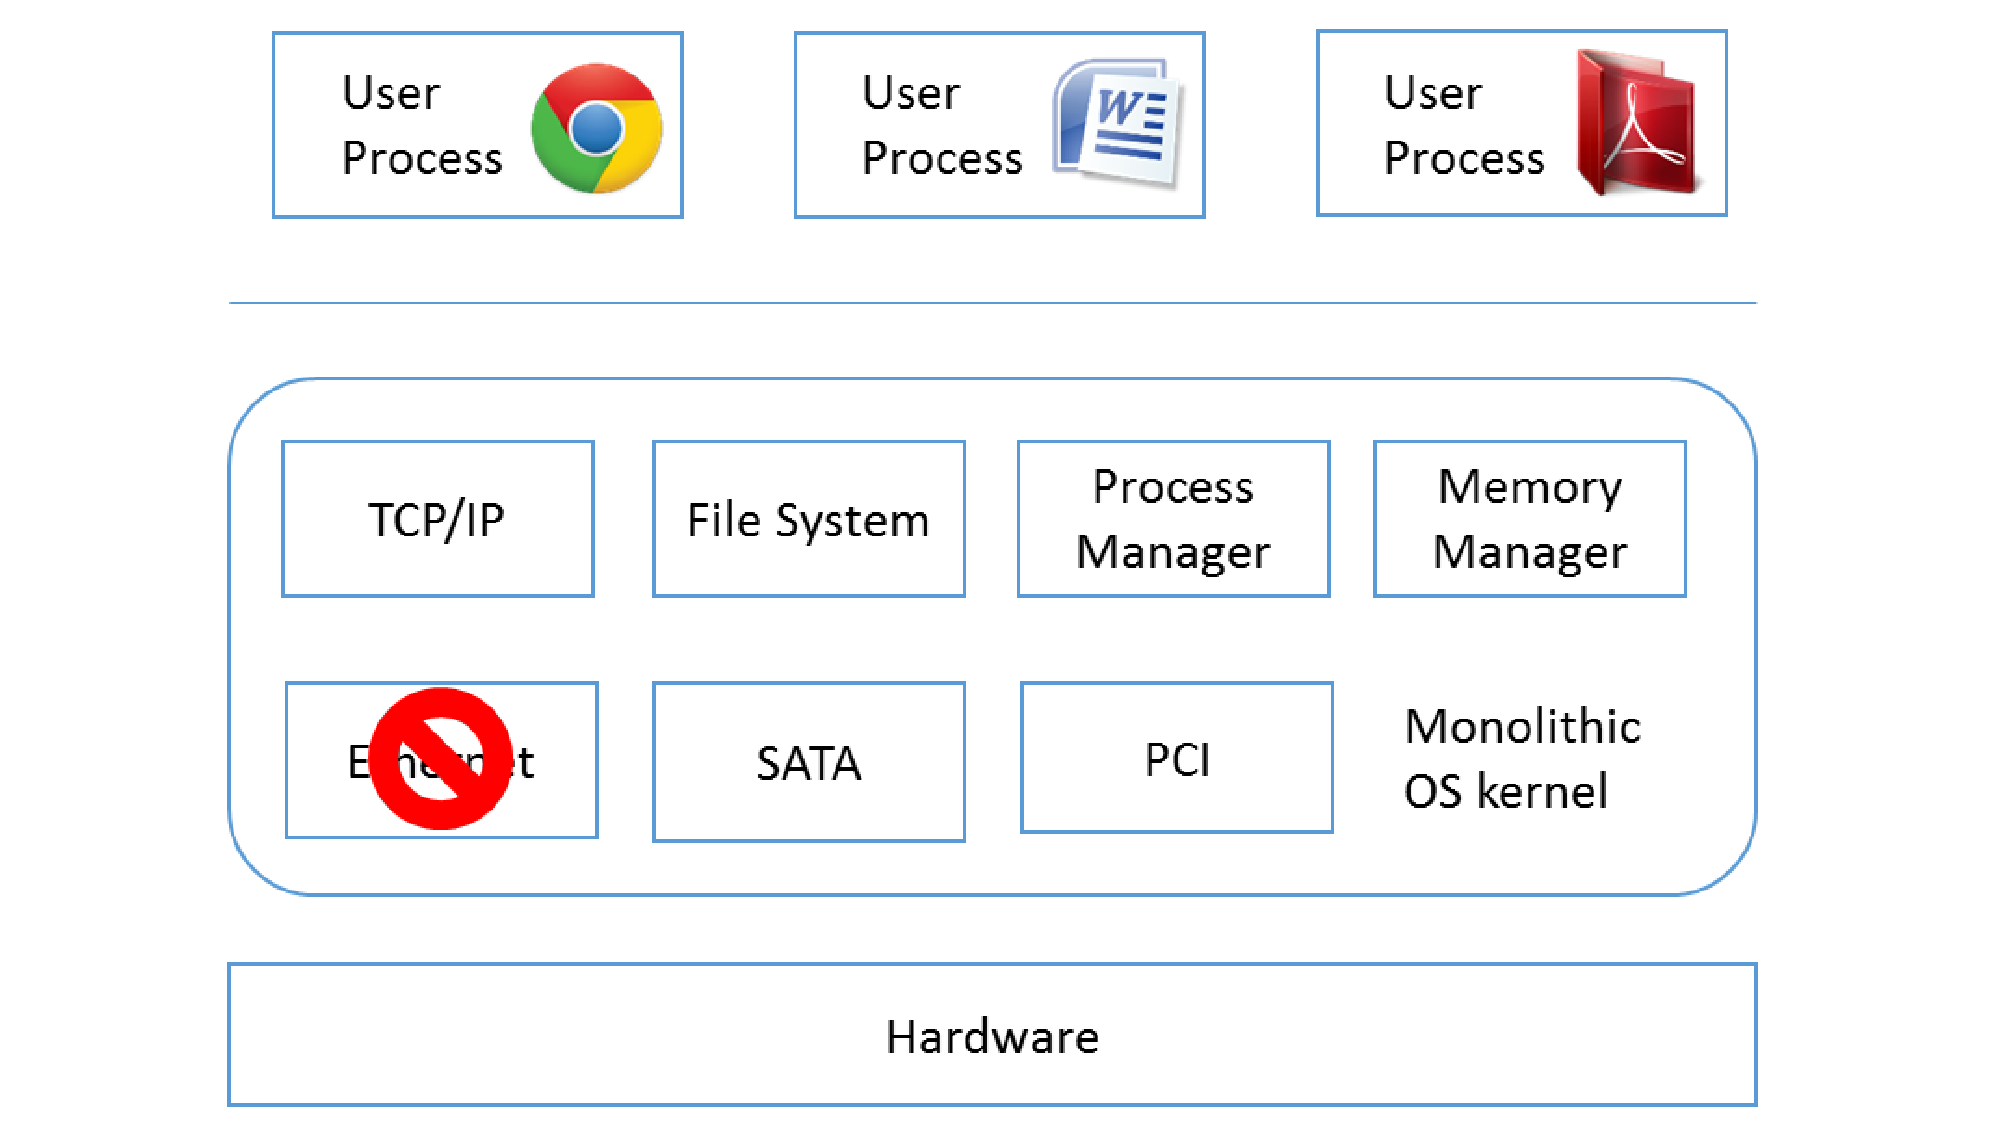
\includegraphics[scale=.25]{kernel-space-1}
	\caption{A kernel component hits a bug}
    \end{subfigure}
	\hfill
    \begin{subfigure}[b]{0.49\textwidth}
	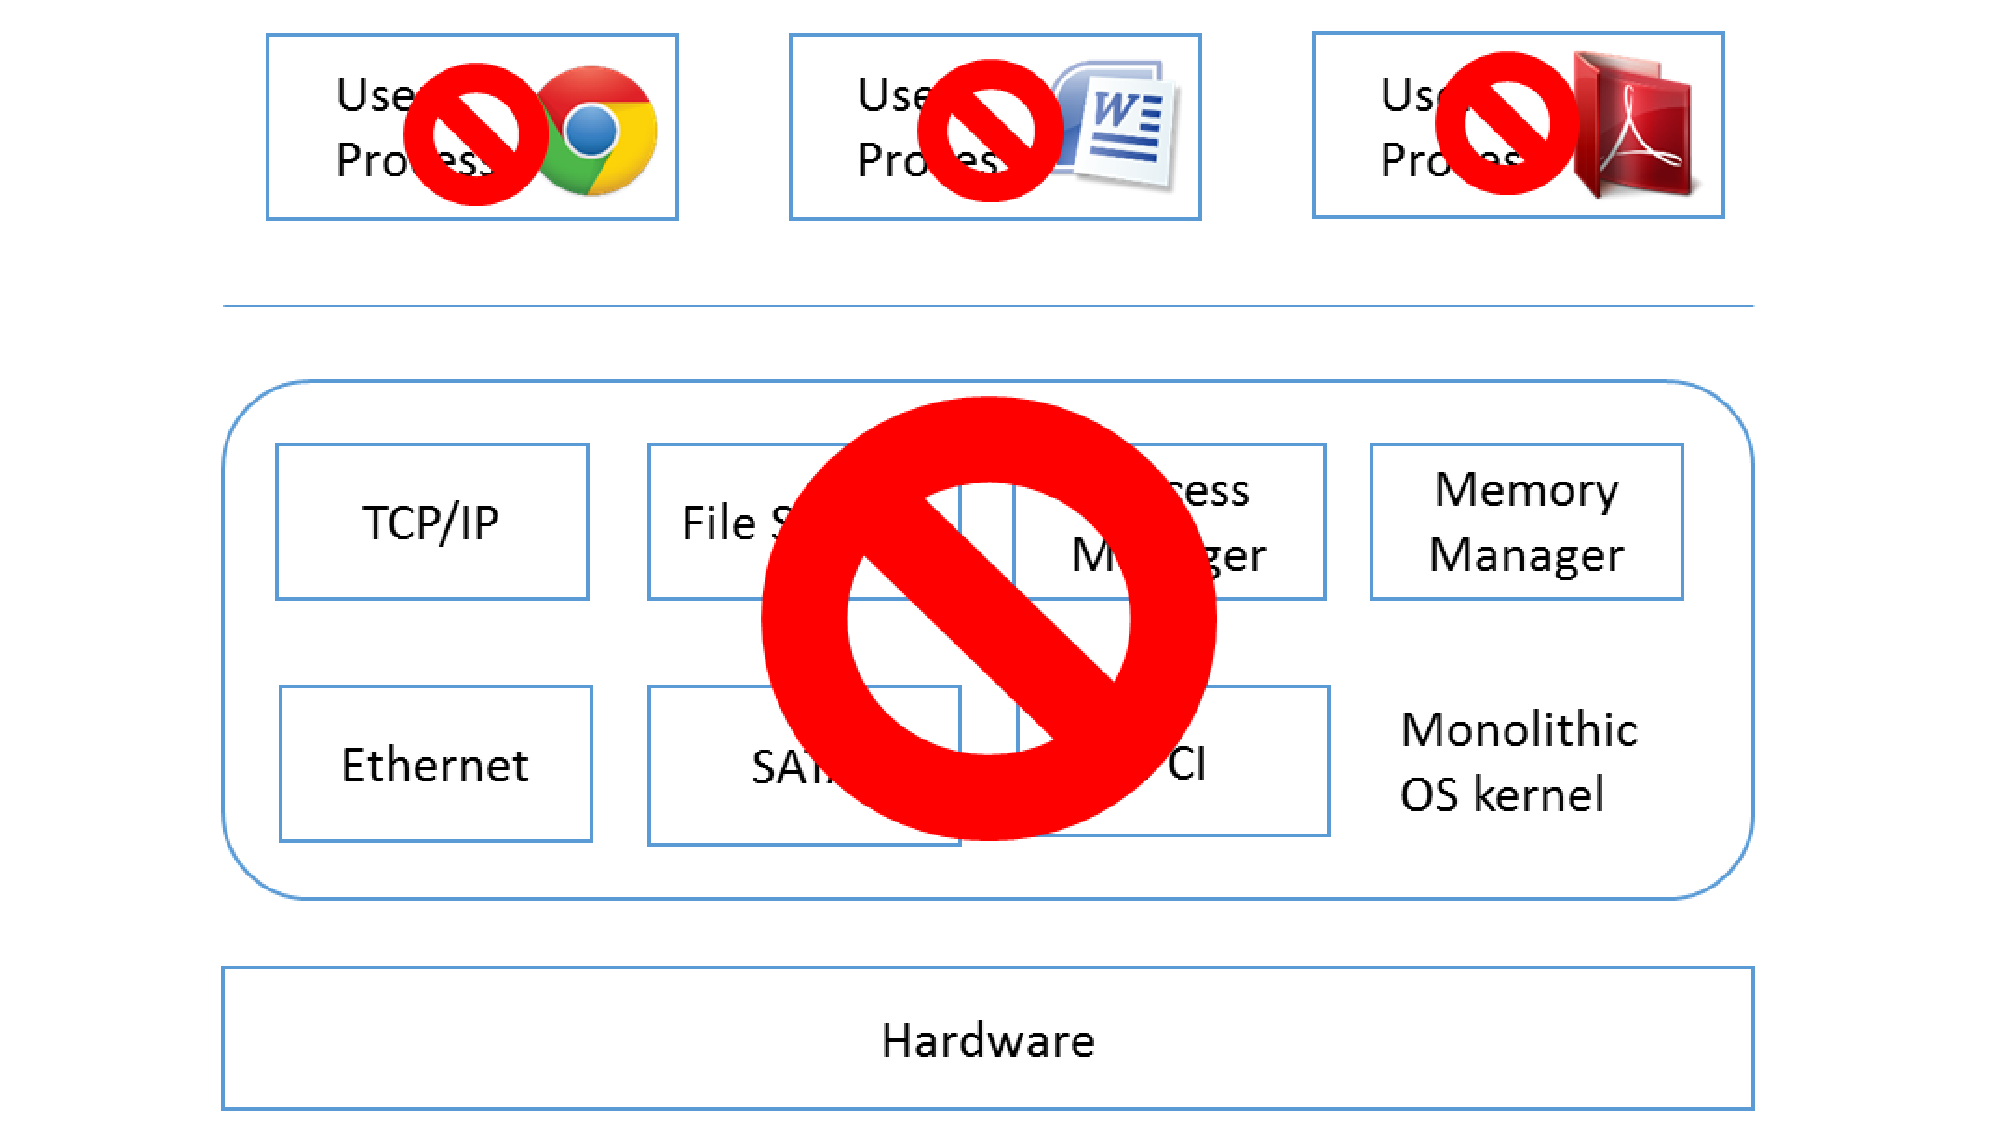
\includegraphics[scale=.25]{kernel-space-2}
	\caption{Results in a system crash}
    \end{subfigure}
    \caption{Kernel level memory protection}\label{fig:Kernel space}
\end{figure}

\section{Virtualization}

Virtualization is the act of creating an abstraction of the hardware of a single machine into several different execution environments. Such abstraction creates the illusion that each separate execution environment is running its own private machine~\cite{Galvin}. 

Virtualization provides the capability to share the underlying hardware resources and still provide an isolated environment to each operating system. Because of this isolation, any failures in an operating system can be contained. Virtualization can be implemented in many different ways, either with or without hardware support. Operating systems might require some changes in order to run in a virtualized environment~\cite{Drepper:2008:CV:1348583.1348591}. It has been shown that virtualization can be utilized to provide better security and robustness for operating systems~\cite{Fraser04safehardware, LeVasseur04UnmodifiedDriverReuse, Riley:2008:GPK:1433006.1433008}.
\begin{figure}[!ht]
    \centering
    \begin{subfigure}[b]{0.49\textwidth}
	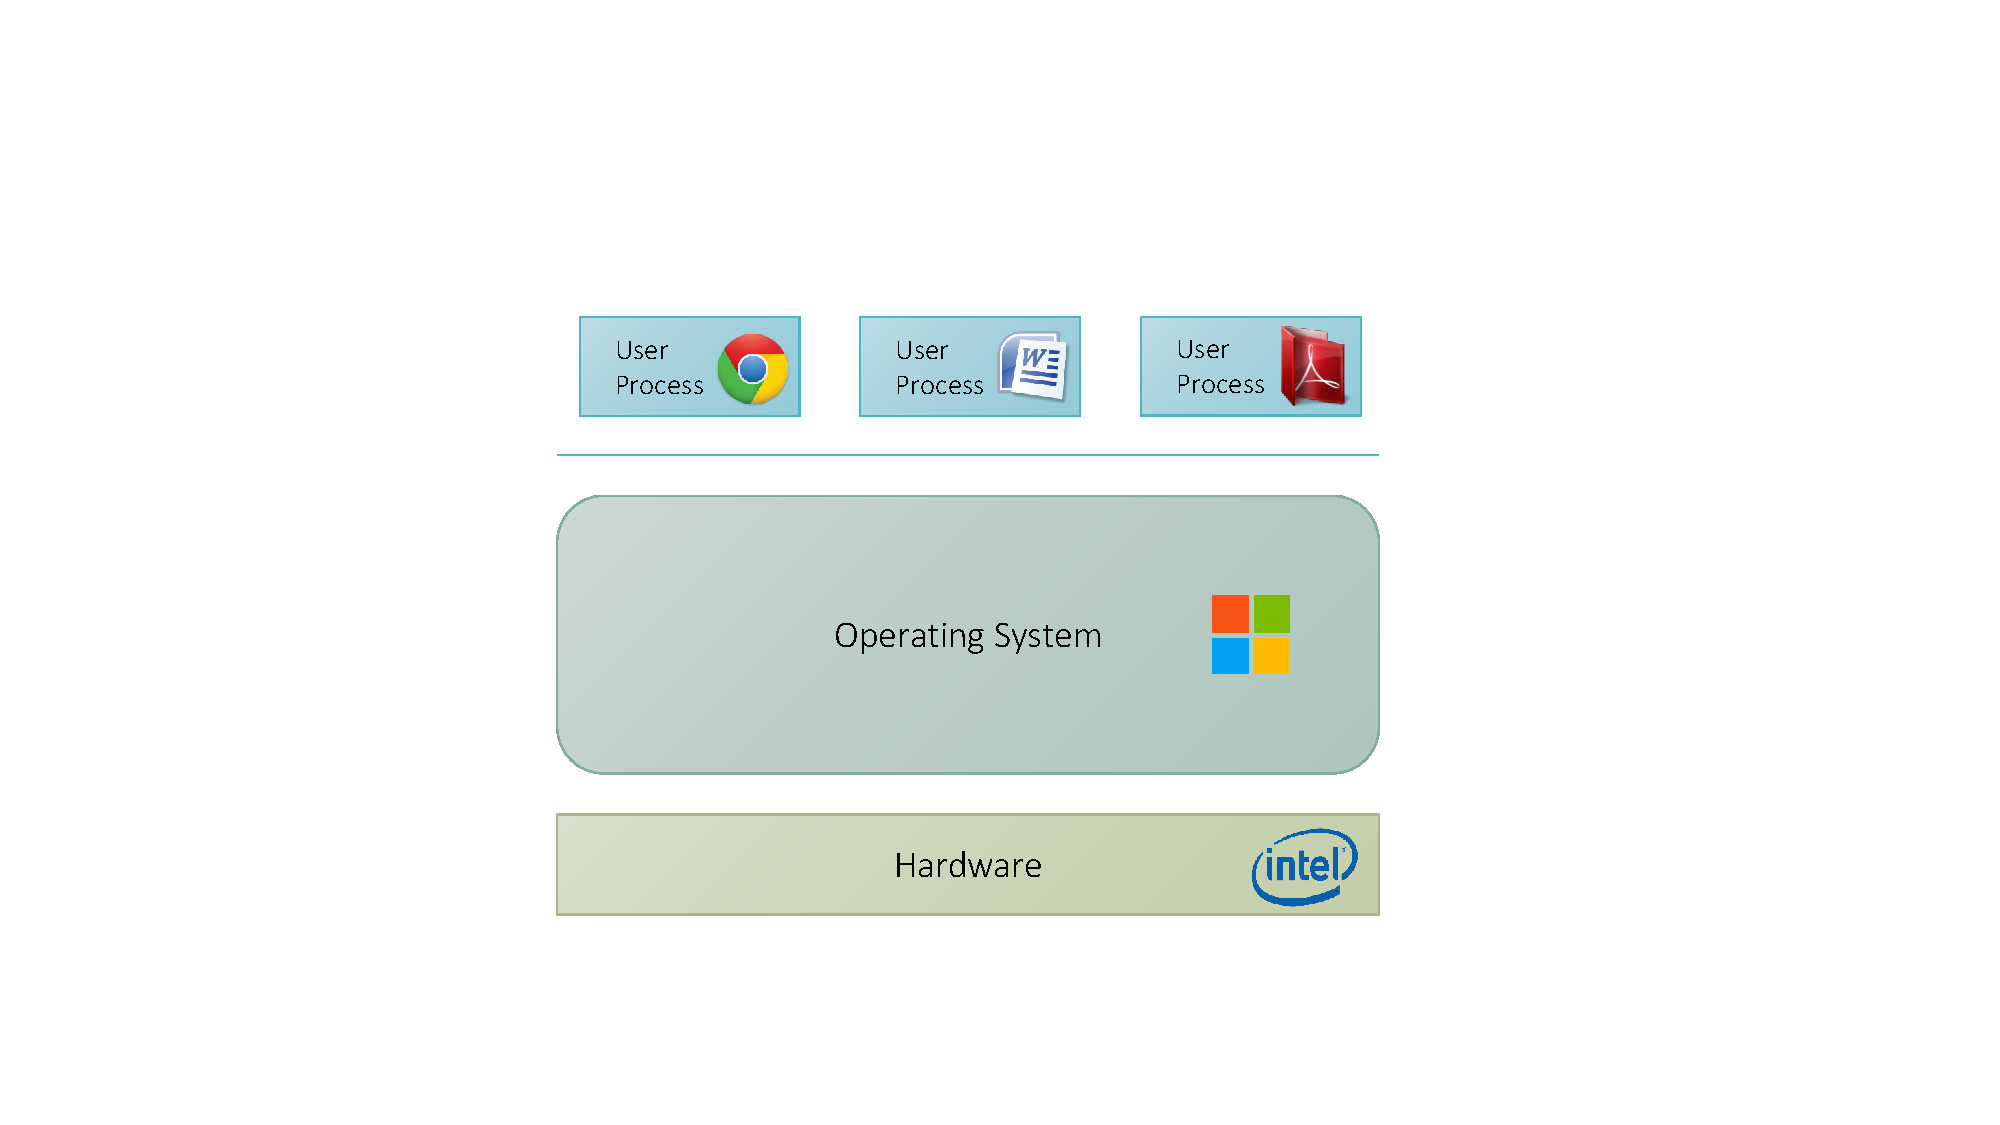
\includegraphics[scale=.25]{OS-arch}
	\caption{Operating System Architecture}
	\label{fig:OS}
    \end{subfigure}
	\hfill
    \begin{subfigure}[b]{0.49\textwidth}
	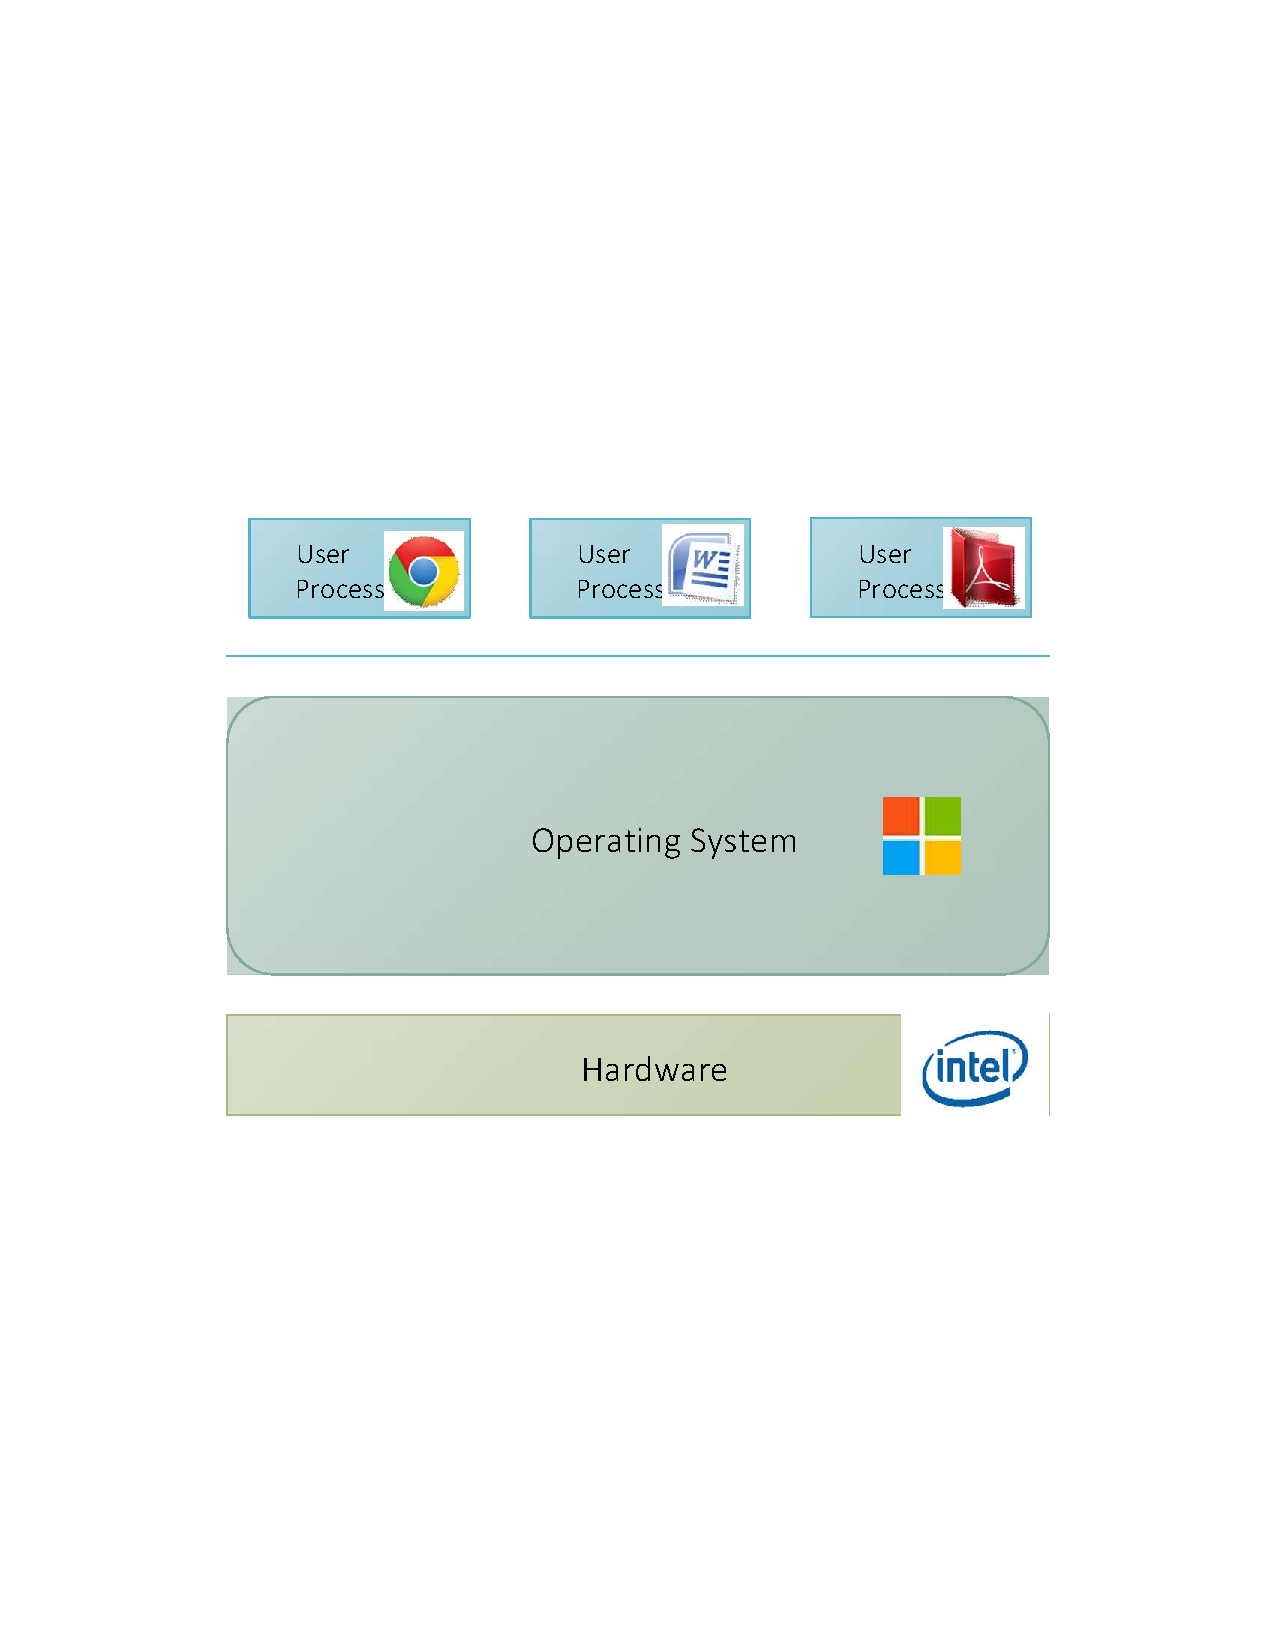
\includegraphics[scale=.25]{virtualization}
	\caption{Virtualization}
	\label{fig:Virtualization}
	\end{subfigure}
    \caption{Comparision of a non-virtualized system and a virtualized system}\label{fig:Kernel space}
\end{figure}

\subsection{Hypervisors}
A hypervisor is a piece of computer software, firmware, or hardware that creates and runs virtual machines. Operating system virtualization is achieved by inserting a VMM between the guest operating system and the underlying hardware. Most of the literature treats VMM and hypervisors synonymously. However, whereas a VMM is a software layer specifically responsible for virtualizing a given architecture, a hypervisor is an operating system that manages VMM. This operating system may be a general purpose one, such as Linux, or it may be developed specifically for the purpose of running virtual machines~\cite{Agesen:2010:EXV:1899928.1899930}.

A computer on which a hypervisor is running one or more virtual machines is defined as a host machine. Each virtual machine is called a guest machine. Multiple instances of a variety of operating systems share the virtualized hardware resources. Among widely known hypervisors are Xen~\cite{barham2003xen, Chisnall:2007:DGX:1407351}, KVM~\cite{Habib:2008:VK:1344209.1344217, kivity2007kvm}, VMware ESXi~\cite{Agesen:2010:EXV:1899928.1899930} and VirtualBox~\cite{camargos2008virtualization}.

There are two types of hypervisors~\cite{Popek:1974:FRV:361011.361073}
\begin{itemize}
\item Type 1 hypervisors are also called native hypervisors or bare metal hypervisors. Type 1 hypervisors run directly on the host's hardware and manage guest operating systems. Type 1 hypervisors represent the classic implementation of virtual-machine architectures such as SIMMON, and CP/CMS. Modern equivalents include Oracle VM Server for SPARC, Oracle VM Server, the Xen hypervisor~\cite{barham2003xen}, VMware ESX/ESXi~\cite{Agesen:2010:EXV:1899928.1899930} and Microsoft Hyper-V.
\begin{figure}[!ht]
\centering
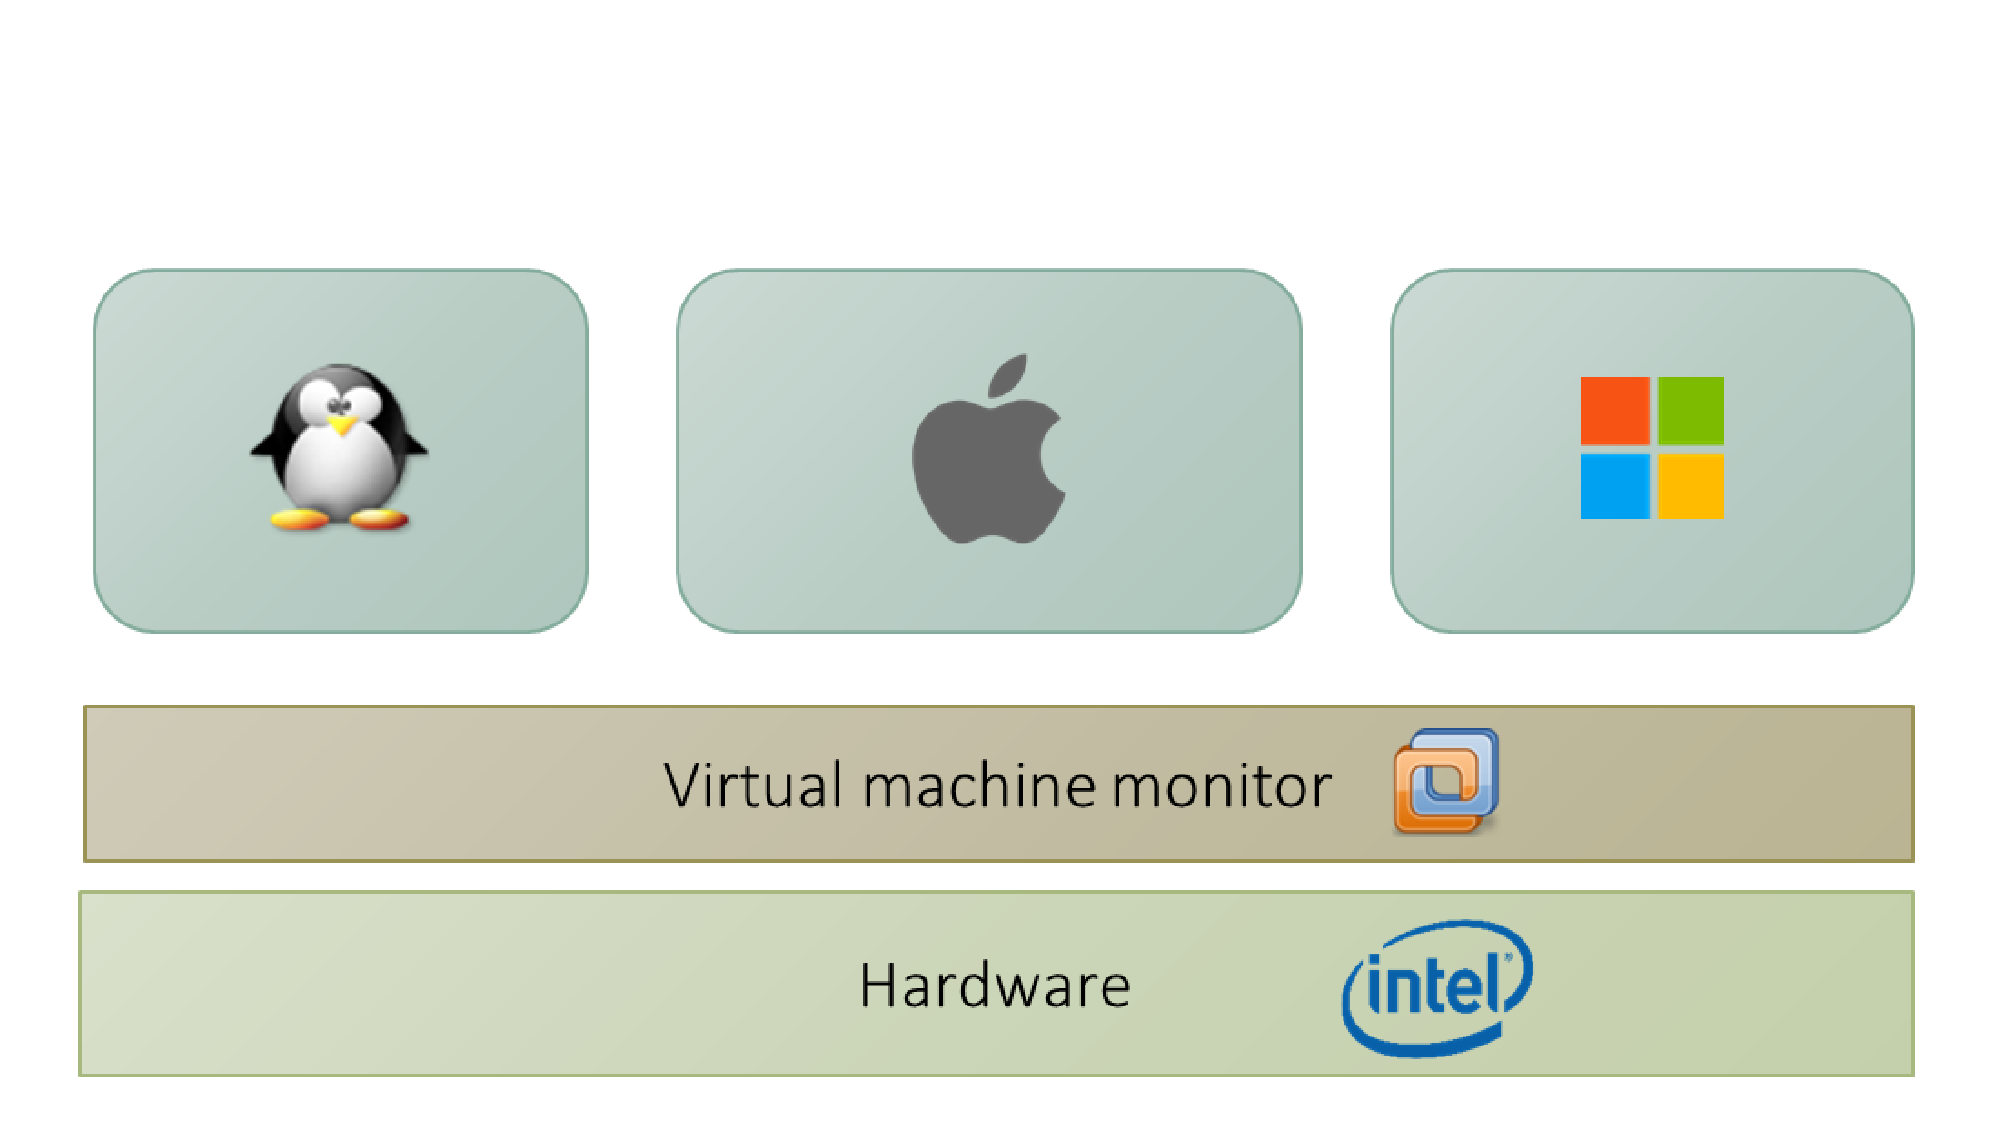
\includegraphics[scale=.35]{type1}
\caption{Type 1 hypervisors}
\label{Type 1 hypervisor}
\end{figure}
\item Type 2 hypervisors are also called hosted hypervisors. Type 2 hypervisors run within a conventional operating-system environment. VMware Workstation and VirtualBox are some examples of Type 2 hypervisors~\cite{Sugerman:2001:VID:647055.715774, camargos2008virtualization}.
\begin{figure}[!ht]
\centering
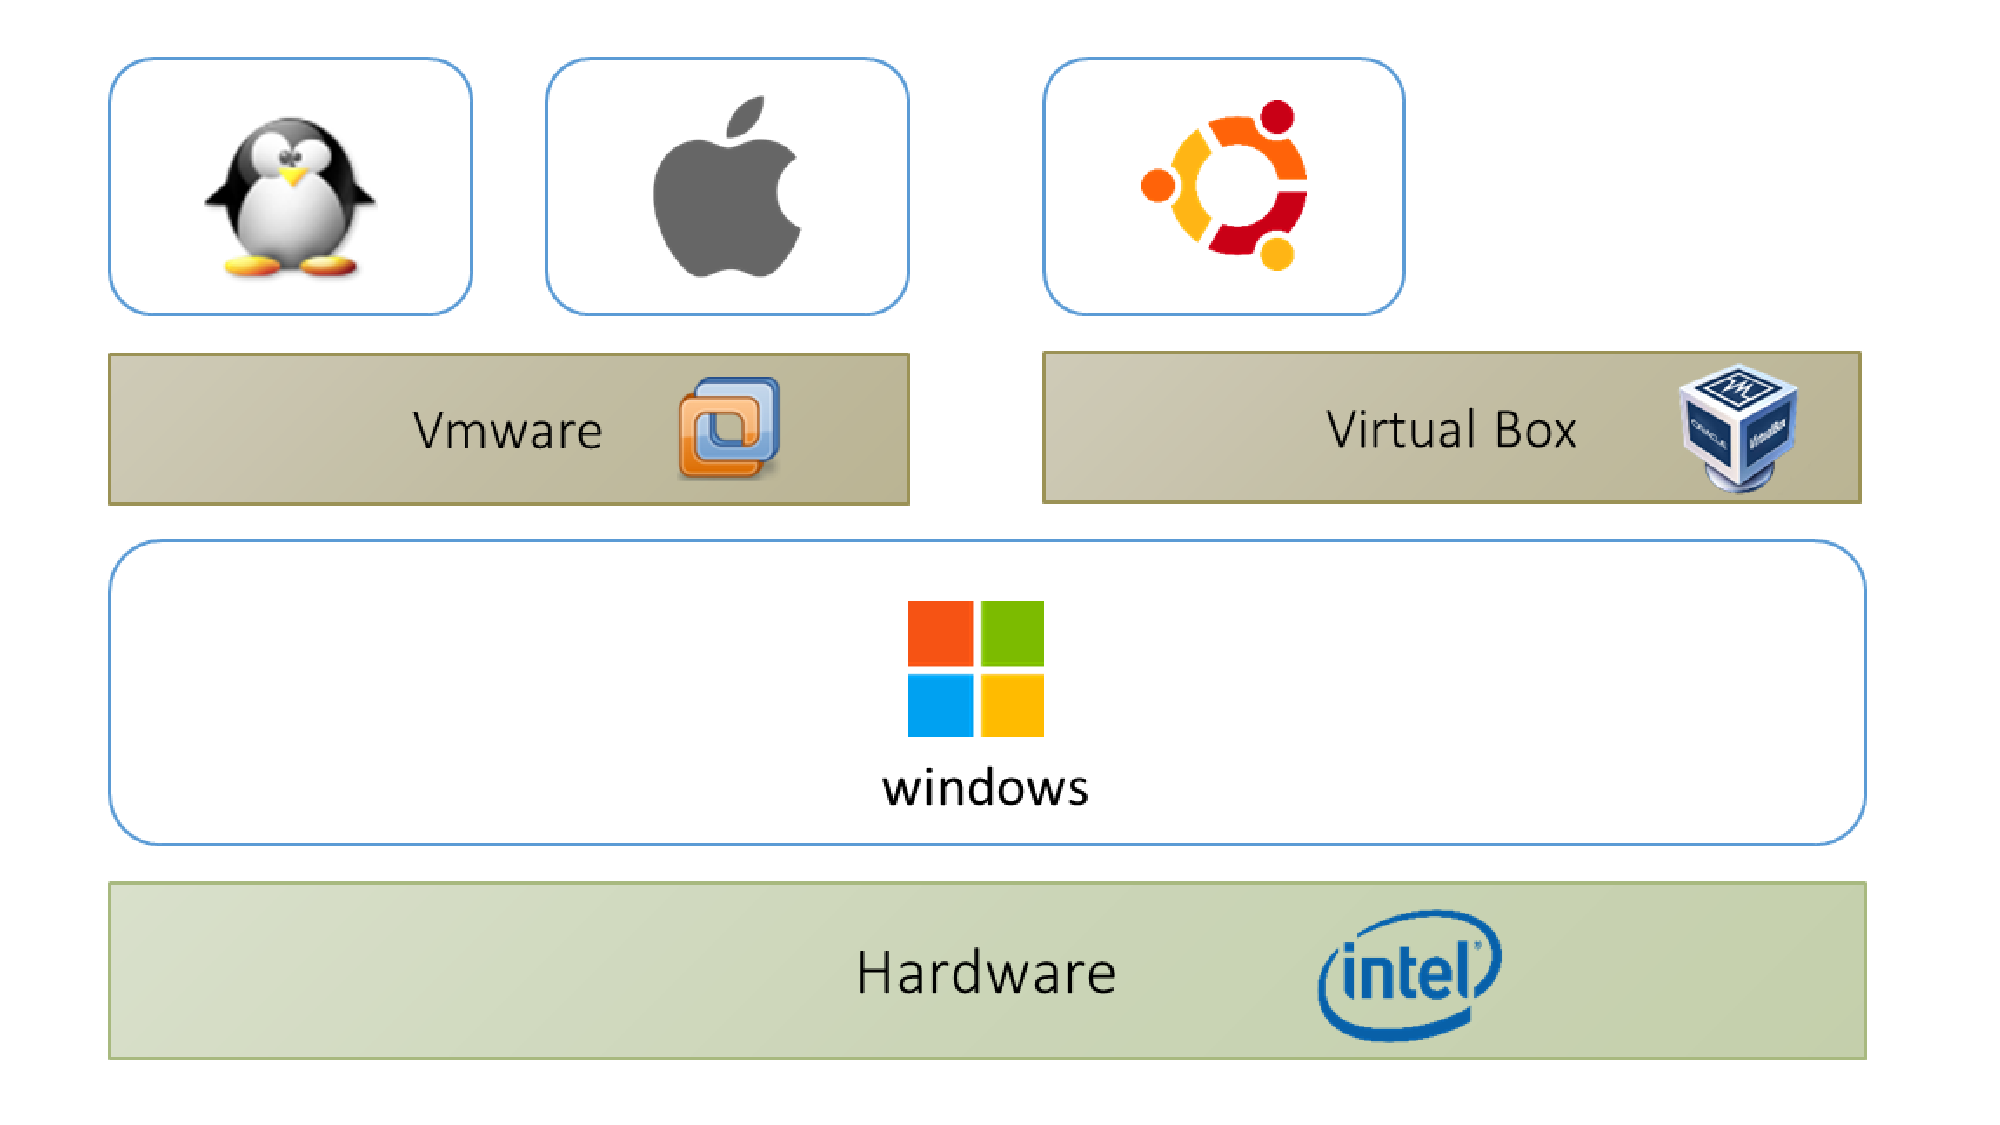
\includegraphics[scale=.4]{type2}
\caption{Type 2 hypervisors}
\label{fig:Type 2 hypervisor}
\end{figure}
\end{itemize}

\subsection{Xen Hypervisor}
Xen~\cite{barham2003xen} is a widely known Type 1 hypervisor that allows the execution of virtual machines in guest domains~\cite{king2003operating}. Xen runs guest operating systems in environments known as domains. \texttt{Domain 0} is the first guest to run, and has elevated privileges. Xen loads a \texttt{domain 0} guest kernel during boot. Unprivileged domain is called \texttt{domain U}. The Xen hypervisor does not include device drivers. Device management is included in privileged \texttt{domain 0}. \texttt{Domain 0} uses the device drivers present in the guest operating system. The other domains access devices using a split device driver architecture, in which a frontend driver in a guest domain communicates with a backend driver in \texttt{domain 0}.

Figure~\ref{xen-split2} shows how an application running in a \texttt{domain U} guest writes data on a physical device. Xen provides an inter-domain memory sharing API accessed through the guest kernel extensions and an interrupt-based inter-domain signaling facility called event channels to implement the efficient inter-domain communication. Split device driver model uses memory sharing APIs to implement I/O device ring buffers to exchange requests and responses across domains and use event channels to send virtual interrupt when requests and responses are shared. 

Consider the example shown in Figure~\ref{xen-split2}. First, write request is sent to the file system. After that the frontend driver puts the data into memory which is shared between \texttt{domain 0} and \texttt{domain U}. The other half of the split device driver called the backend, running in the \texttt{domain 0} guest, reads the data from the buffer and sends it to the real device driver. The data is then written to the actual physical device~\cite{Chisnall:2007:DGX:1407351}.

\begin{figure}[!h]
\centering
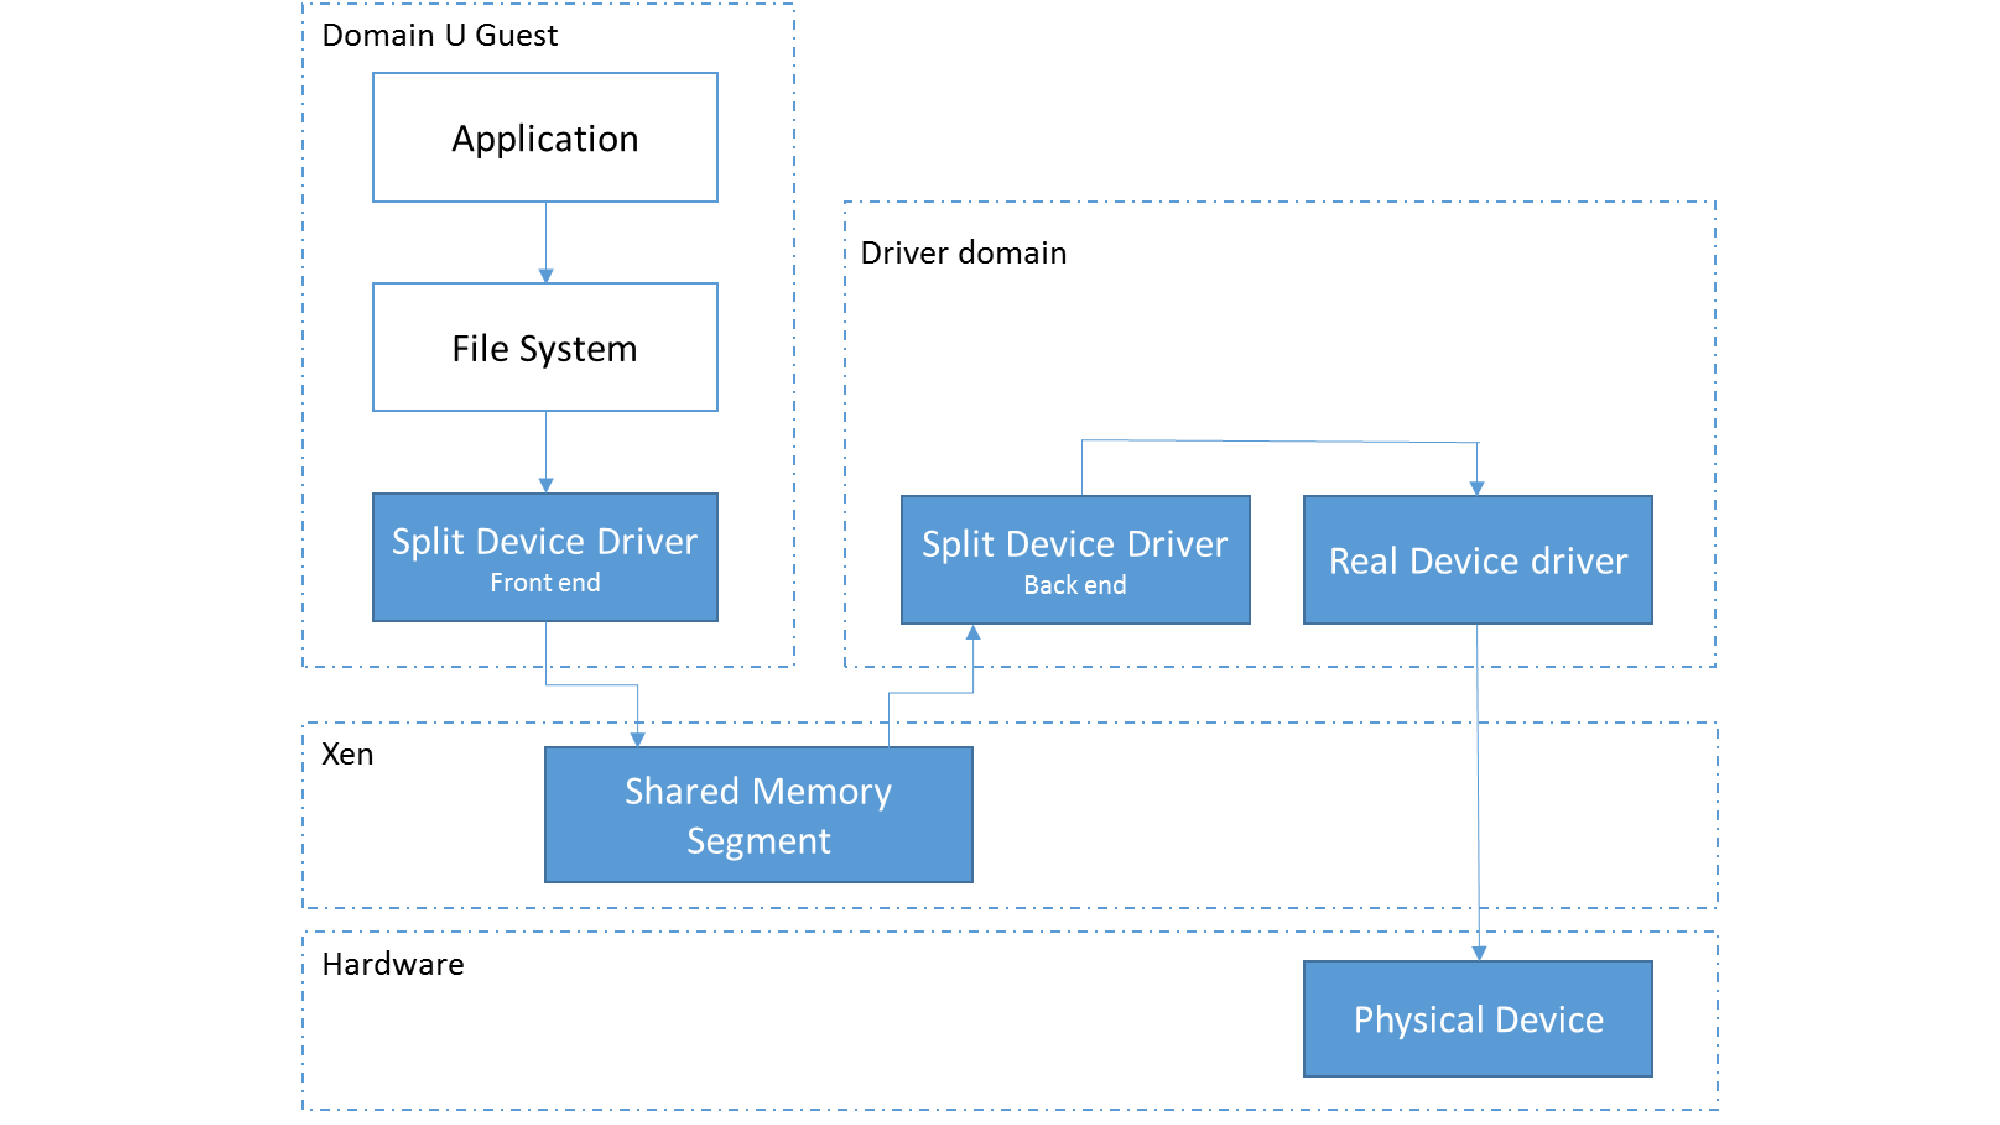
\includegraphics[scale=.50]{xen-split-fs}
\caption{Xen split device driver}
\label{xen-split2}
\end{figure}
\begin{figure}[!h]
\centering
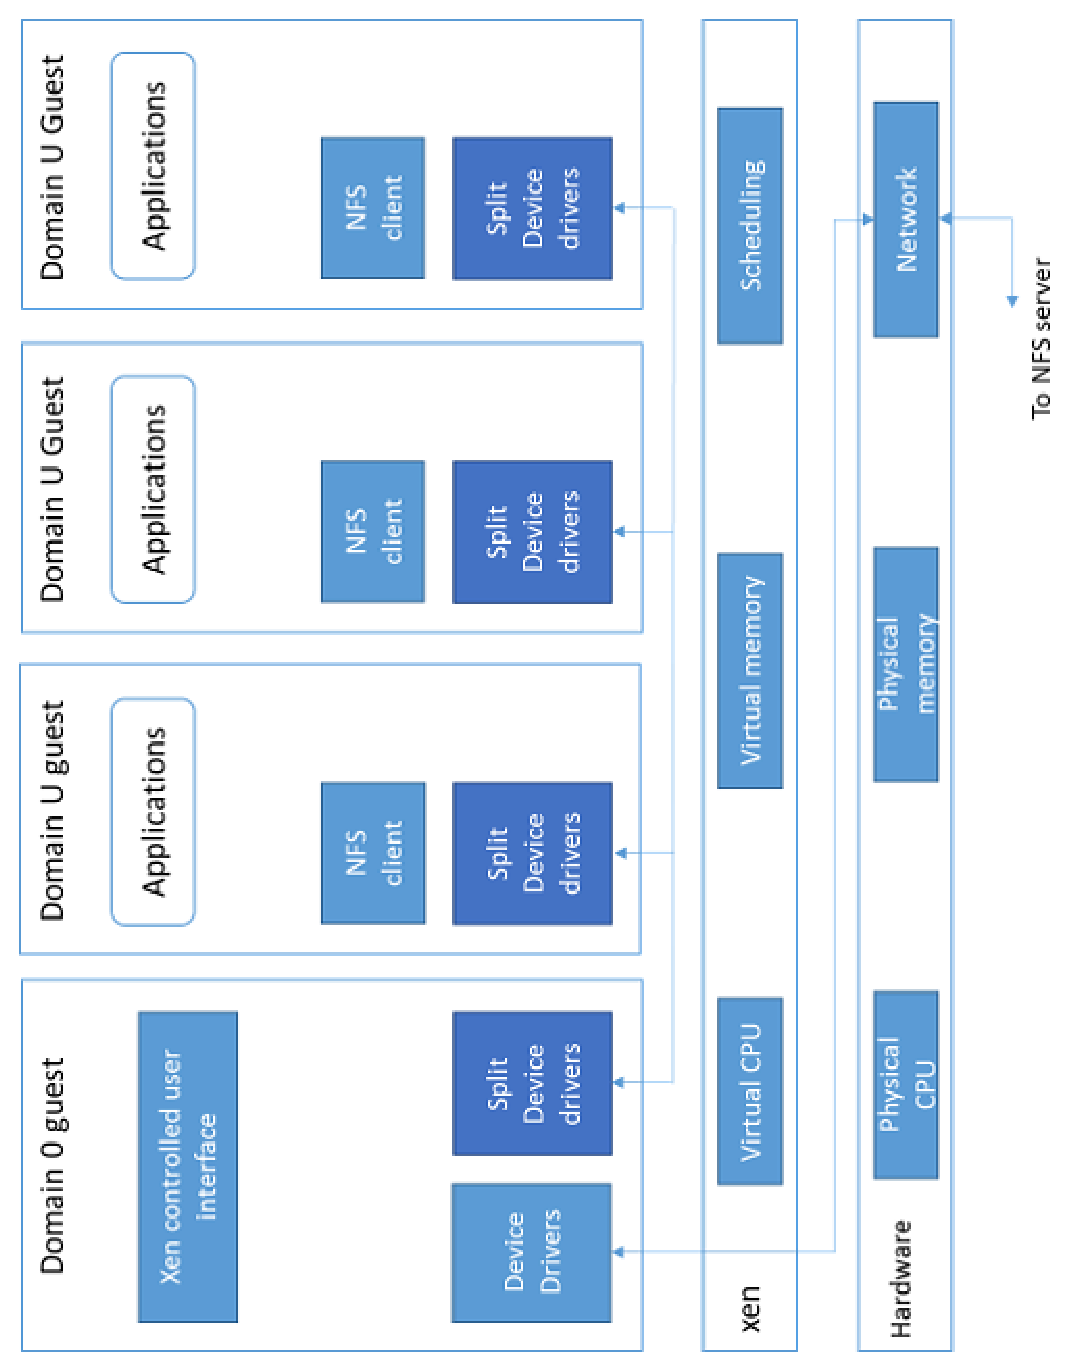
\includegraphics[scale=.50]{xen}
\caption{Xen}
\label{xen}
\end{figure}

\subsubsection*{Hypercalls and Events}
Hypercalls and event channels are the two mechanisms that exist for interactions between the Xen hypervisor and domains. A hypercall is a software trap from a domain to the Xen hypervisor, just as a syscall is a software trap from an application to the kernel~\cite{hypercall}. Domains use hypercalls to request privileged operations like updating pagetables. 

An event channel is to the Xen hypervisor as a signal is to an operating system. An event channel is used for sending asynchronous notifications between domains. Event notifications are implemented by updating a bitmap. After scheduling pending events from an event queue, the event callback handler is called to take appropriate action. The callback handler is responsible for resetting the bitmap of pending events and responding to the notifications in an appropriate manner. A domain may explicitly defer event handling by setting a Xen readable software flag: this is analogous to disabling interrupts on a real processor. Event notifications can be compared to traditional UNIX signals acting to flag a particular type of occurrence. For example, events are used to indicate that new data has been received over the network, or used to notify that a virtual disk request has completed. 

\subsubsection*{Data Transfer: I/O Rings}
\label{subsec:io rings}
Hypervisors introduce an additional layer between a guest OS and I/O devices. Xen provides a data transfer mechanism that allows data to move vertically through the system with minimum overhead. 
\begin{figure}[!ht]
\centering
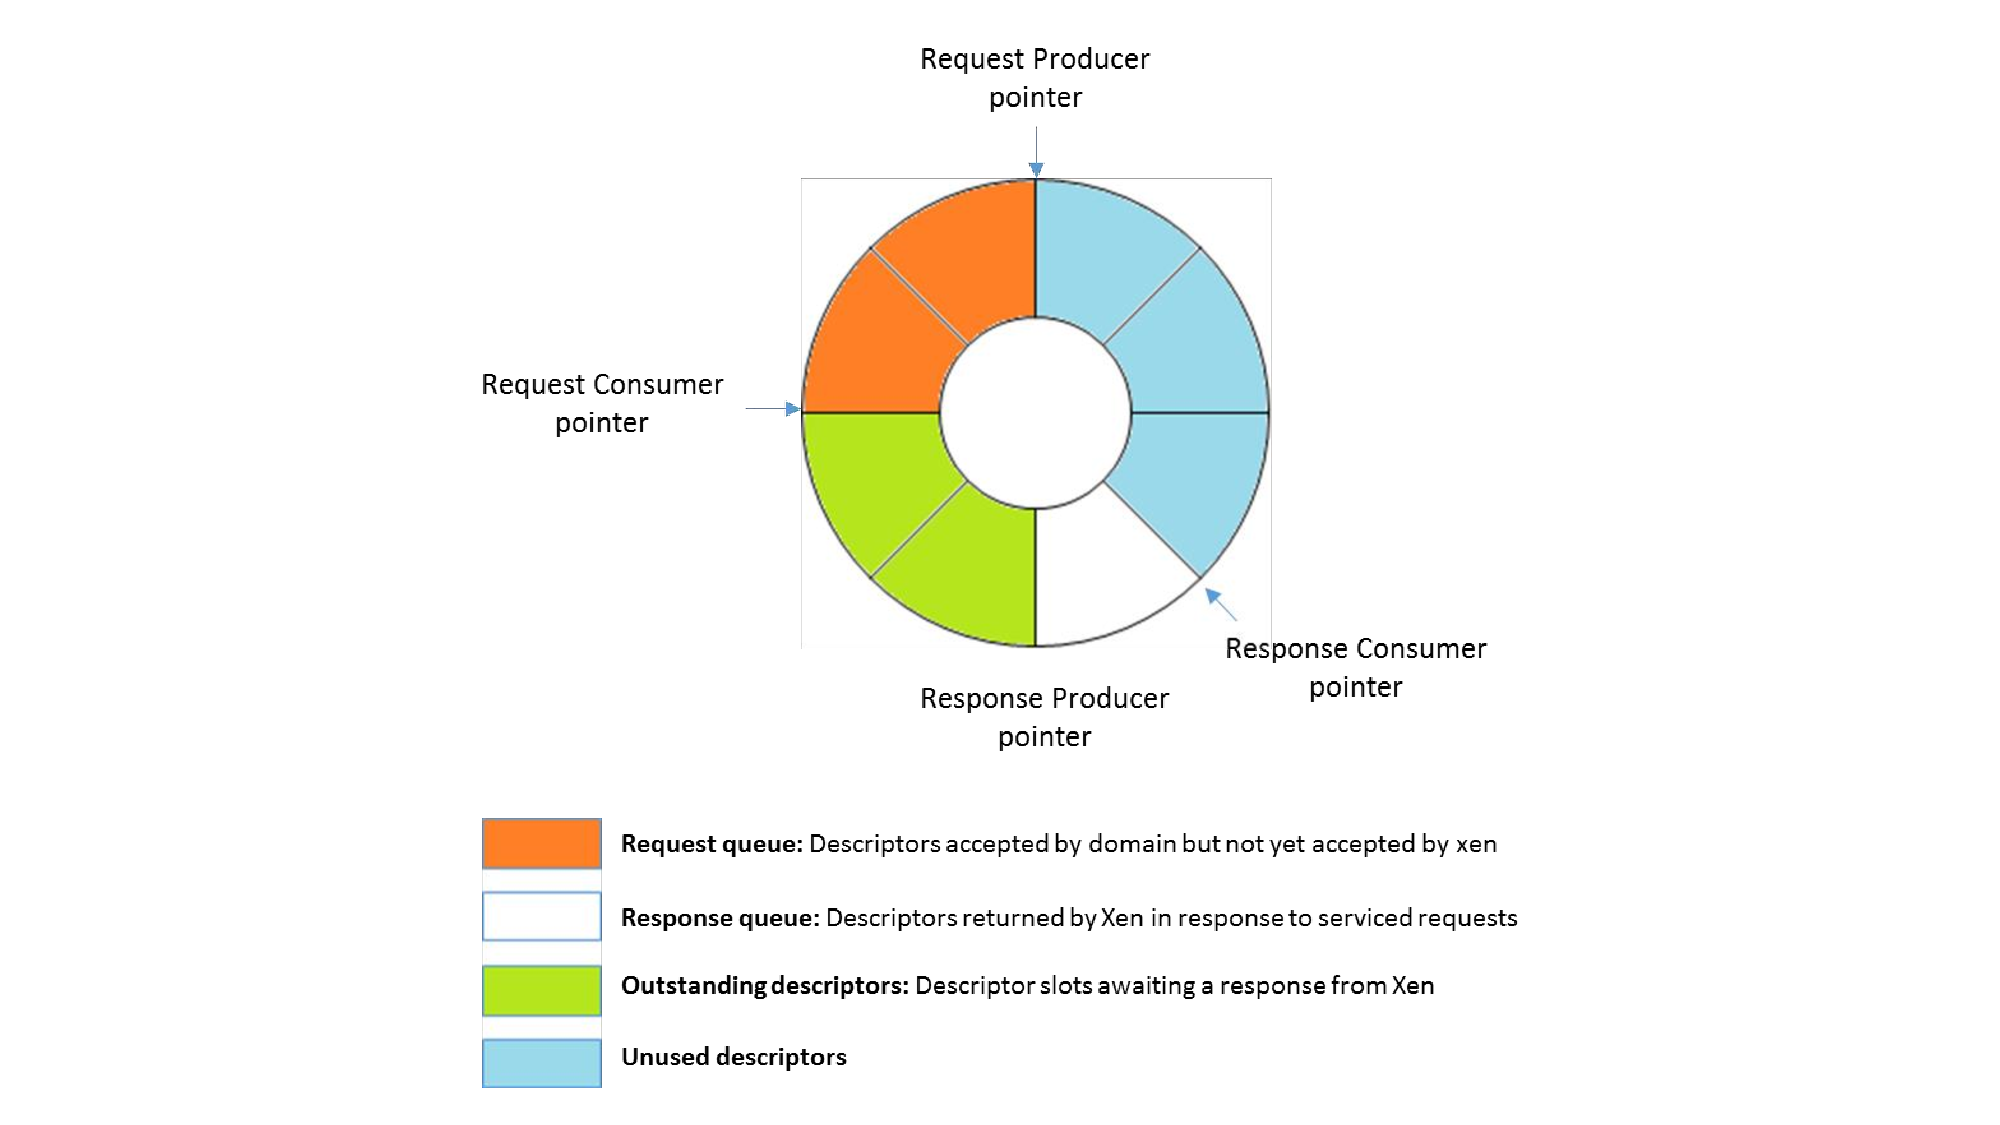
\includegraphics[scale=.5]{IObuffer}
\caption{Ring I/O buffer}
\label{fig:Ring buffer}
\end{figure}

Figure~\ref{fig:Ring buffer} shows the structure of an I/O descriptor ring. An I/O descriptor ring is a circular queue of descriptors allocated by a domain. These descriptors do not contain I/O data. I/O data buffers are allocated separately by the guest OS and are indirectly referenced by these I/O descriptors. Access to an I/O ring is based on two pairs of producer-consumer pointers.
\begin{enumerate}
\item Request producer pointer: A producer domain places requests on a ring by advancing the request producer pointer. 
\item Request consumer pointer: A consumer domain removes these requests by advancing the request consumer pointer.
\item Response producer pointer: A Consumer domain places responses on a ring by advancing the response producer pointer. 
\item Response consumer pointer: A producer domain removes these responses by advancing the response consumer pointer.
\end{enumerate} 

Notifications are not sent for each individual request and response. A domain can enqueue multiple requests and responses before notifying the other domain. This allows each domain to tradeoff between latency and throughput.
\begin{figure}[!ht]
\centering
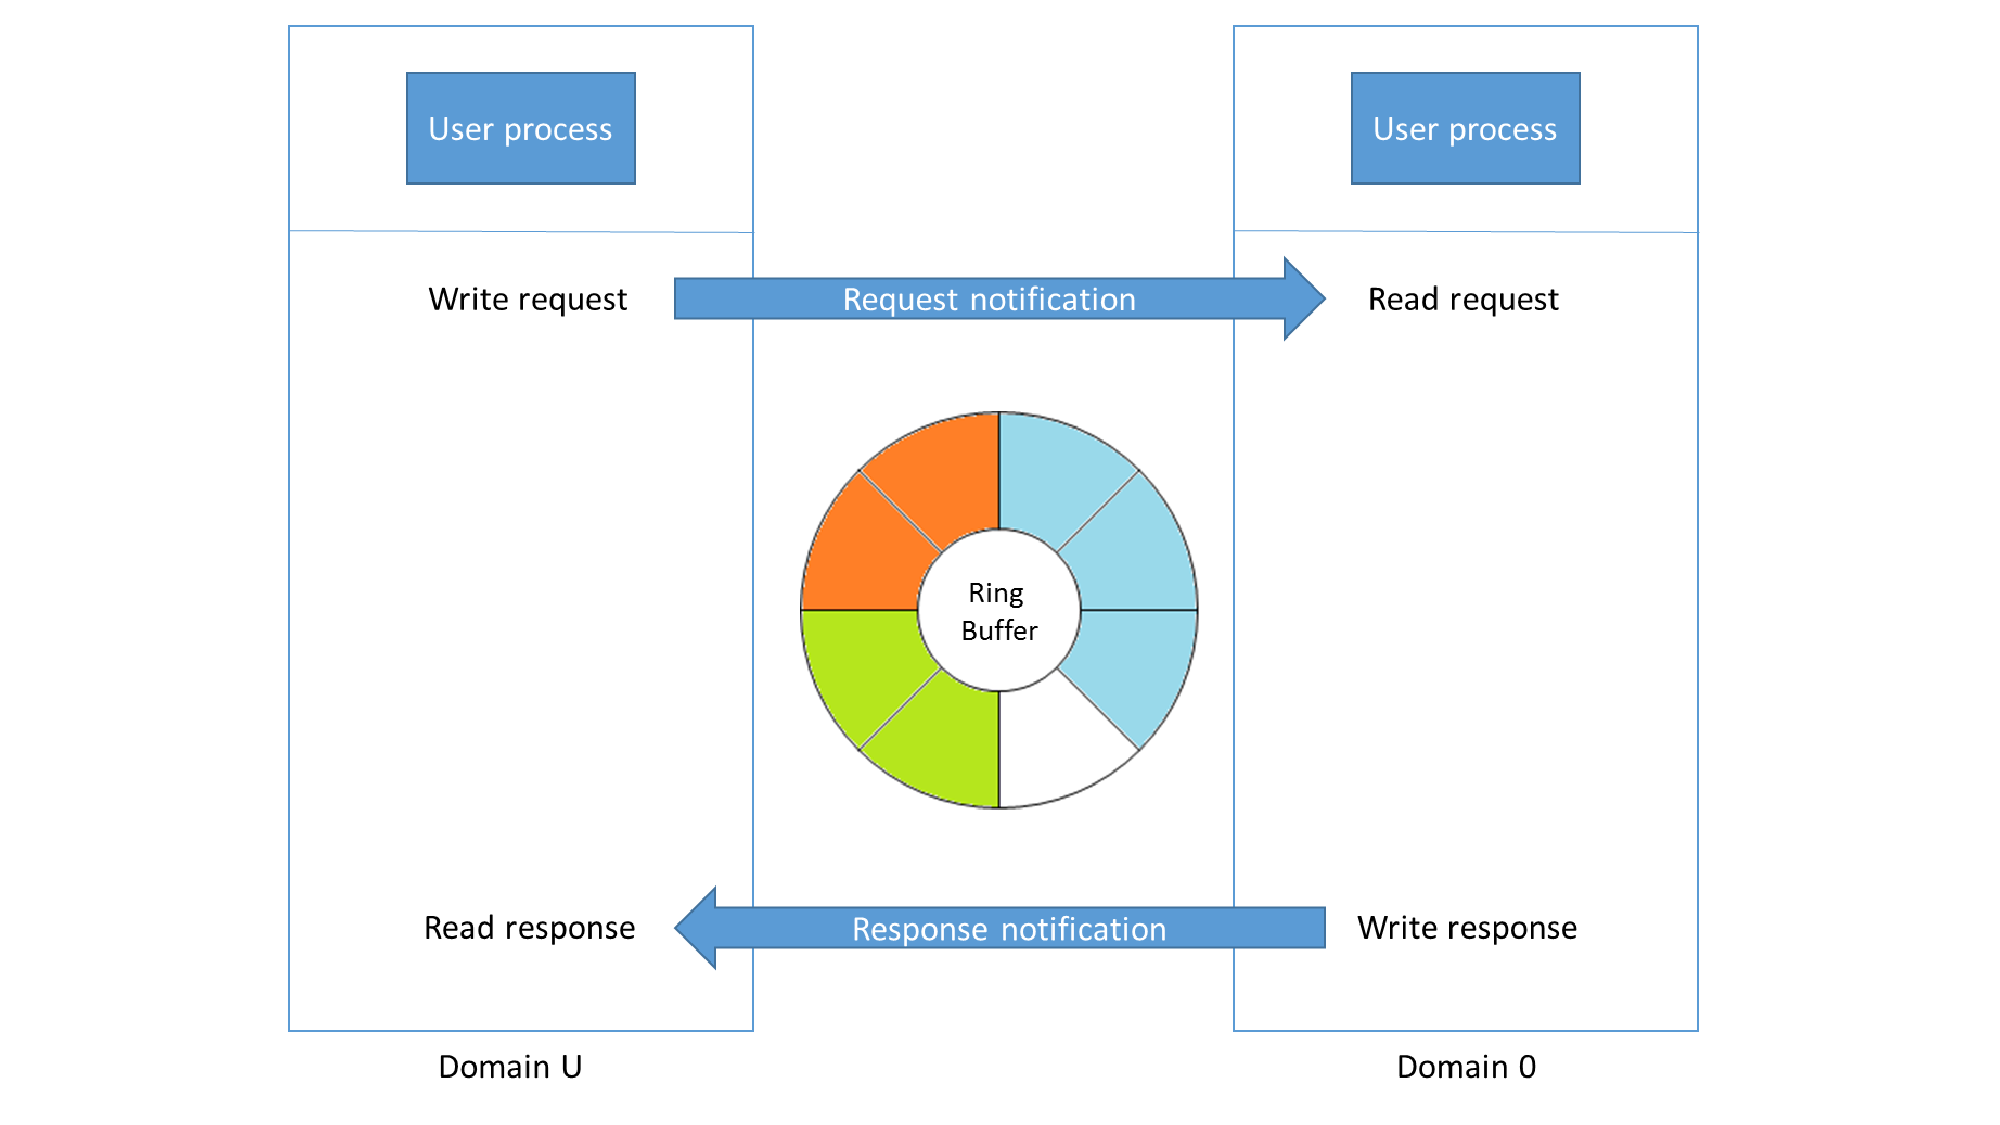
\includegraphics[scale=.5]{IObuffer2}
\caption{Ring I/O buffer}
\label{fig:Ring buffer}
\end{figure}

\subsection*{Shared Pages}
\label{subsec:sharedpages}
\subsubsection*{Grant Table} 
Grant tables are a mechanism provided by the Xen hypervisor for sharing and transferring memory between the domains. It is an interface for granting foreign access to machine frames and sharing memory between unprivileged domains. Each domain has its own grant table data structure, which is maintained by the Xen hypervisor. The grant table data structure is used to verify the access permissions other domains have to pages allocated by a domain~\cite{granttable}.

\subsubsection*{Grant References}
Grant table entries are referred to as grant references. A grant reference entry contains all necessary details about a shared page. 

The Xen hypervisor virtualizes the physical memory. In Xen hypervisor, a domain requires the machine address of a frame in order to share a memory with other domain. It is not possible to know the machine address of a frame for a domain. A grant reference removes the dependency on the real machine address in order to share a page and makes it possible to share the memory between domains.\cite{Chisnall:2007:DGX:1407351, barham2003xen, granttable} 
\ifbool{toShowBibliography}{\bibliography{references}}{}
